\documentclass[12pt,letterpaper]{article}
\usepackage{latexsym}
\usepackage{tikz} % a. Set paper size to Letter, 8½ x 11.
\usetikzlibrary{positioning,arrows.meta,fit,backgrounds}

%\usepackage[letterpaper,top=3.0cm, bottom=3.0cm, footnotesep=1.0cm]{geometry}
\usepackage[letterpaper,margin=1in]{geometry} % e. Set margins of 1 inch (2.54 cm.) on all four sides of the paper. 
\usepackage{mathptmx} % d. ...in a simple roman face except where indicated below (§3). 
\usepackage[singlespacing]{setspace} % Set line spacing to 1 throughout the document
\usepackage{fancyhdr} 

% Set the headheight to at least 14.49998pt
\setlength{\headheight}{14.49998pt}

\usepackage{relsize}

\usepackage[bottom]{footmisc}
\usepackage{tabularx}
    
\pagestyle{empty}

% Set paragraph indentation to 1.5cm
\setlength{\parindent}{2em}


\usepackage{url}
\usepackage{hyperref}
\usepackage[ngerman,english]{babel}

\usepackage{graphicx}

\usepackage[htt]{hyphenat}

%\setmainfont[Mapping=tex-text]{Linux Libertine O} %Falls nicht vorhanden müssen die LinLibertine-ttf-Dateien nach C:\windows\fonts verschoben werden

\usepackage{booktabs}    % For nice-looking tables
\usepackage{longtable}
\usepackage{natbib}      % Citation support (required for crossrefs)
\usepackage{expex}
\bibpunct[:]{(}{)}{;}{a}{}{,} % Defaults for in-text citations
\usepackage{bibentry}    % Print individual references

\usepackage{acronym}
\usepackage{multicol}

\author{Alexander Giller}

\usepackage{scrhack} % Recommended to avoid potential conflicts
\usepackage{microtype}

\usepackage[acronym,xindy,toc]{glossaries}
\makeglossaries
\loadglsentries{pages/glossary.tex} % important update for glossaries, before document

\usepackage{ragged2e}
% Float placement: keep figures and tables close to their text
\usepackage[section]{placeins}   % floats do not drift past the next \section (chapter)
\renewcommand{\topfraction}{0.85}
\renewcommand{\bottomfraction}{0.6}
\renewcommand{\textfraction}{0.1}
\renewcommand{\floatpagefraction}{0.75}
\setcounter{topnumber}{3}
\setcounter{bottomnumber}{2}
\setcounter{totalnumber}{5}
\setlength{\emergencystretch}{3em}
\usepackage{array}
\newcolumntype{P}[1]{>{\raggedright\arraybackslash}p{#1}} % left-aligned paragraph column (no underfull boxes in tables)
\usepackage[htt]{hyphenat} % allow line breaks in \texttt words (e.g. after underscores)  % avoid overfull lines with long \texttt names


% Set up hyphenation rules for the language package when mistakes happen
\babelhyphenation[english]{
an-oth-er
ex-am-ple
}

% vertically centred tilde for TPTP negation in typewriter text (Table fof-syntax)
\newcommand{\tptptilde}{\raisebox{-0.45ex}{\textasciitilde}}

% numbers of the evaluation (generated by scripts/eval_all.py)
% generated by scripts/eval_all.py -- do not edit
\providecommand{\EvalCPU}{12th Gen Intel(R) Core(TM) i7-1255U}
\providecommand{\EvalCores}{12}
\providecommand{\EvalRAM}{8\,GB}
\providecommand{\EvalOS}{Linux 5.15.167.4-microsoft-standard-WSL2}
\providecommand{\EvalPython}{3.12.3}
\providecommand{\EvalLark}{1.3.1}
\providecommand{\EvalVampire}{Vampire 5.0.1 (Release build, commit 1b13eaf on 2026-01-18 12:14:50 +0000)}
\providecommand{\EvalCommit}{10bfb54}
\providecommand{\EvalDate}{2026-10-23}
\providecommand{\EvalReps}{3}
\providecommand{\EvalNValid}{47}
\providecommand{\EvalNInvalid}{53}
\providecommand{\EvalNPrv}{100}
\providecommand{\EvalAccValid}{47}
\providecommand{\EvalRejValid}{0}
\providecommand{\EvalUnknownValid}{0}
\providecommand{\EvalTimeoutValid}{0}
\providecommand{\EvalRejInvalid}{52}
\providecommand{\EvalAccInvalid}{0}
\providecommand{\EvalUnknownInvalid}{1}
\providecommand{\EvalTimeoutInvalid}{0}
\providecommand{\EvalScore}{151}
\providecommand{\EvalMaxScore}{153}
\providecommand{\EvalScorePct}{98.7}
\providecommand{\EvalWrongAcc}{0}
\providecommand{\EvalOffN}{91}
\providecommand{\EvalOffValid}{44}
\providecommand{\EvalOffInvalid}{47}
\providecommand{\EvalOffAccValid}{44}
\providecommand{\EvalOffRejInvalid}{46}
\providecommand{\EvalOffTimeouts}{0}
\providecommand{\EvalOffWrongAcc}{0}
\providecommand{\EvalOffScore}{136}
\providecommand{\EvalOffMaxScore}{138}
\providecommand{\EvalSampleN}{9}
\providecommand{\EvalOffRejValid}{0}
\providecommand{\EvalOffUnknownValid}{0}
\providecommand{\EvalOffUnknownInvalid}{1}
\providecommand{\EvalOffScorePct}{98.6}
\providecommand{\EvalTstAgree}{70}
\providecommand{\EvalTstTotal}{71}
\providecommand{\EvalTstEdge}{5}
\providecommand{\EvalTstWrong}{1}
\providecommand{\EvalTstWrongAcc}{1}
\providecommand{\EvalRulesInSet}{34}
\providecommand{\EvalRulesInternal}{20}
\providecommand{\EvalRulesDelegated}{14}
\providecommand{\EvalDerivedSteps}{15573}
\providecommand{\EvalInternalSteps}{15449}
\providecommand{\EvalInternalPct}{99.2}
\providecommand{\EvalFallbackSteps}{1}
\providecommand{\EvalAtpOnlySteps}{123}
\providecommand{\EvalUnresolvedSteps}{0}
\providecommand{\EvalInternalMedianShare}{50}
\providecommand{\EvalLargestProof}{PRV071+1.s}
\providecommand{\EvalLargestProofSteps}{10005}
\providecommand{\EvalWallMedian}{1.52\,s}
\providecommand{\EvalWallPNinety}{2.06\,s}
\providecommand{\EvalWallMax}{11.00\,s}
\providecommand{\EvalOverTen}{1}
\providecommand{\EvalTimeouts}{0}
\providecommand{\EvalRssMedian}{26}
\providecommand{\EvalRssMax}{172}
\providecommand{\EvalAtpShare}{8.6}
\providecommand{\EvalAtpCalls}{54}
\providecommand{\EvalAtpMean}{252\,ms}
\providecommand{\EvalAtpMedian}{80\,ms}
\providecommand{\EvalInterpStart}{1.40\,s}
\providecommand{\EvalNoAtpMedian}{1.42\,s}
\providecommand{\EvalExtRunsN}{109}
\providecommand{\EvalExtRunsValid}{35}
\providecommand{\EvalExtRunsInvalid}{66}
\providecommand{\EvalExtRunsAgree}{101}
\providecommand{\EvalExtRunsFalseRej}{0}
\providecommand{\EvalExtRunsWrongAcc}{0}
\providecommand{\EvalExtRunsScore}{167}
\providecommand{\EvalExtRunsWallMedian}{1.45\,s}
\providecommand{\EvalSuboptimal}{1}
\providecommand{\EvalParseErrors}{1}
\providecommand{\EvalScoreBinary}{153}
\providecommand{\EvalOffScoreBinary}{138}
\providecommand{\EvalScoreTernary}{151}
\providecommand{\EvalUncertainCount}{1}
\providecommand{\EvalNoAtpVerifiedValid}{22}
\providecommand{\EvalNoAtpWrongAcc}{0}
\providecommand{\EvalNoAtpScoreBinary}{94}
\providecommand{\EvalNoAtpScoreTernary}{106}
\providecommand{\EvalNoAtpUncertain}{27}
\providecommand{\EvalNoAtpWallMedian}{1.41\,s}
% generated by scripts/eval_all.py -- do not edit
\providecommand{\EvalIntSteps}{155}
\providecommand{\EvalIntAccYes}{146}
\providecommand{\EvalIntAccNo}{0}
\providecommand{\EvalIntRejYes}{2}
\providecommand{\EvalIntRejNo}{4}
\providecommand{\EvalIntUnknown}{3}
\providecommand{\EvalIntAtpMedian}{68\,ms}
\providecommand{\EvalIntAtpMax}{9.97\,s}
% generated by scripts/eval_all.py -- do not edit
\providecommand{\EvalMutN}{361}
\providecommand{\EvalMutKilled}{303}
\providecommand{\EvalMutEq}{58}
\providecommand{\EvalMutMiss}{0}
\providecommand{\EvalMutRate}{100.0}
\providecommand{\EvalMutProofs}{43}

% generated by scripts/eval_all.py -- do not edit
\providecommand{\EvalInputsN}{10}
\providecommand{\EvalInputsAccepted}{1}
\providecommand{\EvalInputsCrash}{3}
% generated by scripts/eval_all.py -- do not edit
\providecommand{\EvalExtraN}{109}
\providecommand{\EvalExtraValid}{35}
\providecommand{\EvalExtraInvalid}{66}
\providecommand{\EvalExtraEdge}{8}
\providecommand{\EvalExtraAccOk}{35}
\providecommand{\EvalExtraRejOk}{66}
\providecommand{\EvalExtraByRule}{66}
\providecommand{\EvalExtraEdgeRej}{6}
\providecommand{\EvalExtraEdgeAcc}{2}
\providecommand{\EvalExtraRules}{20}
% generated by scripts/eval_all.py -- do not edit
\providecommand{\EvalCheckerLines}{2856}
\providecommand{\EvalCheckerCov}{87.2}
\providecommand{\EvalTotalCov}{90.4}
\providecommand{\EvalBiggestChecker}{\texttt{skolem\_checker}}
\providecommand{\EvalBiggestLines}{619}
\providecommand{\EvalSmallestChecker}{\texttt{existential\_gen\_checker}}
\providecommand{\EvalSmallestLines}{74}
\providecommand{\EvalMainLines}{1231}


\begin{document}
\pagenumbering{roman} % front matter: i, ii, ... (avoids duplicate page anchors)

\selectlanguage{english}

\begin{center}\uppercase{Ludwig-Maximilians-Universität München}\end{center}
\iflanguage{english}{
\begin{center}\uppercase{Chair of Theoretical Computer Science and Theorem Proving}\end{center}
}
{}

\vspace*{10mm}
\begin{center}

\includegraphics[height=40mm]{sigillum.png}
\end{center}
\vspace*{10mm}

\iflanguage{english}{
%%%Block Englisch:
\title{Designing a Competitive Proof Verification System
for TPTP-Style Benchmarks}
\date{\vspace{-3ex}}
{\let\newpage\relax\maketitle}
\thispagestyle{empty}

\begin{center}
\begin{large}
\begin{Large}
 Master's Thesis\\
\end{Large}
Computer Science\\
\end{large}
\end{center}
\vspace{1cm}
\begin{center}
\begin{large}
Supervisor: Prof. Dr. Jasmin Blanchette\\
\end{large}
\end{center}
\begin{center}
\begin{large}
Advisor: Tanguy Bozec\\
\end{large}
\end{center}
%%%Ende Block Englisch
}{}

\begin{center}
\begin{large}
\iflanguage{english}{
Submission Date: \today \\
}
{}
\end{large}
\end{center}

\vspace{1,5cm}
\cleardoublepage{}

\thispagestyle{empty}
\null
\newpage

\thispagestyle{empty}
\vspace{15mm}
\noindent
\makeatletter
\begin{center}
    \iflanguage{english}{
        {\normalfont\bfseries} Disclaimer
    }{}
\end{center}

\vspace{15mm}

\begin{flushleft}
    \iflanguage{english}{
    I confirm that this Master's thesis was written independently by me, only with the support of the auxiliary tools listed below.
    All passages taken from literature or other sources are appropriately acknowledged and referenced in the text.
    }{}

\vspace{15mm}

\noindent
Munich, \today \hspace{50mm} Author
\end{flushleft}

\vspace{15mm}

\noindent
\iflanguage{english}{
\textbf{Note on the Use of AI Tools}

Artificial intelligence (AI) tools, including large language models
(LLMs) such as Claude Sonnet 5.5, were used in the preparation of this
thesis to support translation and linguistic editing, including
improvements to grammar, spelling, clarity, and overall readability.
In addition, AI-based tools were used for code completion, data
analysis, and the generation of figures and visualizations.

All AI-generated or AI-assisted outputs were reviewed and critically
evaluated by the author. The author takes full responsibility for
the accuracy, interpretation, and final presentation of the content
of this thesis.
}{}

\makeatother

\cleardoublepage{}

\thispagestyle{empty}
\null
\newpage

%\thispagestyle{empty}

\vspace*{20mm}

\begin{center}
\makeatletter

\iflanguage{english}{
{\normalfont\bfseries} Acknowledgments
}
{}
\iflanguage{german}{
{\normalfont\bfseries} Danksagungen
}
{}
\makeatother
\end{center}

\vspace{10mm}

%TODO: Acknowledgments

\cleardoublepage{}
\section*{Abstract}

Modern automated theorem provers are very effective, but whether their results can be trusted depends on an independent check of the proof objects they produce.
This thesis presents the design and implementation of a Python-based proof verifier for TPTP/TSTP derivations, developed according to the specifications of ProoVer 2026, a proof-checking competition held as part of the FLoC Olympics 2026 in Lisbon~\citep{proover-competition}.

In proof verification, a wrongly accepted proof is by far the worst outcome, and the scoring scheme of the competition reflects this: a wrong acceptance costs ten times as much as a correct acceptance gains~\citep{proover-competition}.
The ruleset of ProoVer 2026 also prescribes a three-valued verdict, with \emph{VerifiedGood} for a valid proof, \emph{VerifiedBad} for an invalid proof, and \emph{Unknown} if the checker could not reach a definite conclusion.
A fourth answer, \emph{Timeout}, is given if the verifier does not finish within the time limit of 30 seconds.
The verifier developed in this thesis accepts a proof only if every step has been validated, rejects it only if it has found a concrete defect, and answers \emph{Unknown} in all other cases.
This policy is implemented as a modular pipeline of parsing and normalization, structural and dependency checks, and rule-specific inference checks.
Structural, propositional, quantifier, and clausal rules as well as Skolemization are checked internally, and every failing step gets its own diagnostic.
All remaining steps are passed to an external prover, in this thesis, Vampire, which only sees the premises of the step and never the proof as a whole.

Of the \EvalOffN{} problem/proof pairs provided by the competition committee, the verifier accepts all \EvalOffValid{} valid proofs, rejects \EvalOffRejInvalid{} of the \EvalOffInvalid{} invalid proofs, and answers \emph{Unknown} for the remaining one.
The median run time of \EvalWallMedian{} per proof is well within the limit of 30 seconds wall clock time~\citep{proover-competition}.
This gives \EvalOffScore{} of \EvalOffMaxScore{} points, and no proof is wrongly accepted.
The same holds for the \EvalSampleN{} proofs of the originally published set of 100 that were not scored in the competition.
A generated suite of \EvalExtraN{} rule-level test proofs and \EvalMutN{} mutants of valid proofs, in which every mutant that is no longer valid is rejected, suggests that the checks are not simply tuned to the benchmark.
Even when the external prover is removed, the verifier accepts no invalid proof.
The contributions of this thesis are a soundness argument, a modular verification architecture, a working implementation of the verifier, and an empirical analysis of its performance and robustness under simulated competition conditions.

\textbf{Keywords}: Automated Theorem Proving, Proof Verification, TPTP, TSTP, Fail-Closed Checking, Skolemization, ProoVer 2026.


\newpage
\tableofcontents
\newpage

\pagenumbering{arabic} % main text starts at page 1
\pagestyle{fancy}
\fancyhf{}
\fancyhead[R]{\thepage}
\renewcommand{\headrulewidth}{0pt} %obere Trennlinie

\section{Introduction}
\label{sec:introduction}

\subsection{Motivation}
\label{subsec:motivation}

Automated theorem proving (ATP) is a key technology and finds use in a widespread field ranging from formal reasoning in mathematics to software verification and also in knowledge-based systems~\citep{HandbookAR2001}.
As ATP systems grow more complex, they also become more likely to contain bugs, so that a simple answer such as ``the conjecture is a theorem'' is hard to trust completely.
A common countermeasure is to let the prover generate a derivation, also called a \emph{proof object}, that justifies its answer step by step, and to validate this generated \emph{proof object} with a separate and much simpler program, the \emph{proof checker}/\emph{proof verifier}.
As a consequence trust is moved from a large, fast-changing and hard to understand prover to a small and well-understood checker, an idea that goes back to the de Bruijn criterion and the LCF approach of interactive theorem proving (Section~\ref{subsec:atp-certification}).

In the TPTP ecosystem~\citep{Sut24}, derivations are exchanged in the TSTP format~\citep{Sut10, Sut07-CSR}.
A TSTP derivation is a directed acyclic graph of formulas, where each node records the previous inference rule that produced it and the premises it depends on.
The provers that use the TPTP format can vary in the rules they use, in how precisely they annotate steps, and in how they treat various transformations such as clausification and Skolemization.
A proof checker, which aims to verify the proof objects of such provers, must be sound, meaning that it should never accept an invalid step, while also covering all the rules that occur in real prover outputs and staying within strict time and memory limits.
The established checker for TSTP derivations is GDV~\citep{Sut06-FLAIRS, Sut06, Sut06-CASC-J3, Sut06-CASC}, which verifies each inference step by calling trusted external ATP systems and interpreting their returned outputs~\citep{Sut08-KEAPPA}.
This makes it general, and really reliable, but also slow and highly dependent on these external ATP systems.
The approach of modern checkers therefore includes treating frequent rules and transformations internally and rejecting wrong steps with model finders (Chapter~\ref{sec:related-work}).

ProoVer 2026, the first edition of a competition for proof checkers, held as part of the FLoC Olympics 2026 in Lisbon~\citep{proover-competition}, turns this setting into a benchmark.
Like the CASC competition for provers~\citep{Sut16}, it is based on the TPTP ecosystem, but the systems under evaluation are checkers, instead of provers, and it is also only focused on first-order logic (FOF) problems.
The checkers receive a FOF problem and a TSTP proof, some of which intentionally contain subtle errors, and must classify the proof as valid or invalid, or abstain, if they are not able to decide definitively.
The scoring scheme is strongly asymmetric: a wrongly accepted proof costs ten times as much as a correctly accepted proof gains.
A checker that cannot decide a step therefore faces a real choice between accepting, rejecting, and abstaining, and the existing checkers give no systematic account of how to make it.

\subsection{Research Questions and Scope}
\label{subsec:rq}

The objective of this thesis is to design and implement a Python-based verifier for TSTP derivations that is sound and competitive.
\emph{Sound} means that each accepted inference step is justified by the formal semantics of its rule, whereas \emph{competitive} means that the verifier achieves a high total score under the ProoVer 2026 scoring scheme (Section~\ref{subsec:req-scoring}) within the per-proof 30 second wallclock time limit.
The scope is limited to FOF problems and the inference rules that occur in the ProoVer 2026 benchmarks.
The task, the scoring scheme, and the resource limits are described in Chapter~\ref{sec:requirements} and the thesis focuses on three main research questions.

\begin{description}
  \item[RQ1] Which inference rules and formula fragments must a verifier support to cover the ProoVer 2026 benchmarks? \emph{Measure:} share of steps that are validated internally, by the external prover, or not at all.
  \item[RQ2] How can a modular architecture keep the trusted part of the verifier small while remaining adaptable? \emph{Measure:} size and test coverage of the individual checkers, and the places in the code that must be changed to add a rule.
  \item[RQ3] How do correctness, running time, and memory consumption behave on realistic and on malformed or inconsistent derivations? \emph{Measure:} score, verdict matrix, and run time on the benchmark set and on mutated proofs.
\end{description}

\subsection{Contributions and Structure}
\label{subsec:contributions}

The contributions of this thesis are:
(i) a verdict policy for proof checking that is derived from the competition's scoring scheme and results in a three-valued, fail-closed verdict, under which a proof is accepted only if every step has been validated with true (Chapters~\ref{sec:requirements} and~\ref{sec:design})
(ii) a modular proof checking pipeline for TSTP derivations with internal rule-checking for specific rules, a specific Skolemization check, and a restricted fallback to the external prover Vampire otherwise, together with the Python implementation and diagnostics that recognize failed steps and help solve the occurring issues (Chapters~\ref{sec:design} and~\ref{sec:implementation}) and
(iii) an evaluation on the ProoVer 2026 benchmarks and a suite of mutated proofs showing that the verifier reaches \EvalOffScore{} of \EvalOffMaxScore{} points on the \EvalOffN{} proofs of the competition committee, with no wrong acceptance and a median run time of \EvalWallMedian{} per proof, together with an analysis of the remaining limitations (Chapters~\ref{sec:evaluation} and~\ref{sec:discussion}).

The thesis is structured as follows.
Chapter~\ref{sec:background} introduces first-order logic, the TPTP/TSTP formats, and the ProoVer2026 competition in detail, while Chapter~\ref{sec:related-work} discusses related work, like the other Checkers of the competition, the existing established GDV checker and the used external ATP Vampire.
Chapter~\ref{sec:requirements} derives the requirements for the proof verifier and Chapters~\ref{sec:design} and~\ref{sec:implementation} present the architecture and its implementation.
Following this comes the Chapter~\ref{sec:evaluation}, which shows and evaluates the experimental results.
Chapter~\ref{sec:discussion} discusses implications and limitations of this thesis, and Chapter~\ref{sec:conclusion} answers the research questions and concludes with a potential view into future work and possible room for improvement.

\section{Background}
\label{sec:background}

This chapter introduces the technical foundations of the thesis and the conditions set by the competition.
Section~\ref{subsec:atp-certification} explains why proof certification is needed.
Section~\ref{subsec:verifier-def} then defines what a \emph{proof verifier} is and which properties it should have.
Sections~\ref{subsec:fol} and~\ref{subsec:normal-forms} recall first-order logic and the normal-form transformations that can appear in derivations, in particular Skolemization, which is central to the ProoVer 2026 benchmarks.
Section~\ref{subsec:tptp-tstp} introduces the concrete formats of the TPTP world, namely the first-order language (FOF), the format of derivations (TSTP), and the SZS ontologies used in the competition.
Section~\ref{subsec:proof-objects-soundness} combines the two views and shows under which conditions a checked derivation proves its conjecture.
Section~\ref{subsec:gdv} describes GDV, the established derivation verifier of the TPTP ecosystem, and Section~\ref{subsec:proover2026} explains the ProoVer 2026 competition and its benchmark ruleset.

%==============================================================================
\subsection{Automated Theorem Proving and Proof Certification}
\label{subsec:atp-certification}

Automated theorem provers search for formal derivations that show that a logical statement is valid or that a set of formulas is unsatisfiable.
Their search procedures combine many techniques, for example saturation, clause selection heuristics, and indexing, and are therefore very complex.
For first-order logic, the dominant systems are saturation provers based on resolution \citep{Robinson1965} and superposition, such as Vampire \citep{RiazanovVoronkov2002} and E \citep{SchulzCV2019}.
They are developed and compared in the yearly CASC competition, where Vampire in particular has dominated for many years. It has won the FOF division many times and, in 2025, all eight divisions of CASC-30~\citep{Sut16,CASC30}.
Trusting such a system blindly is difficult, because a single implementation error can lead to a wrong answer without any visible sign. The formal verification of proofs from the higher-order prover Leo-III, for example, uncovered several bugs in the prover \citep{taprogge2026formal}.

The most common answer to this problem is proof verification, which separates \emph{proof search} from \emph{proof checking}.
A prover, like Vampire, generates a proof object, and an independent checker validates each inference step against a trusted set of rules.
The most important property of a checker is \emph{soundness}, which means that it never accepts an invalid proof as valid.
A checker that could do so would make every result that relies on it unreliable.
The checker should also be much simpler than the prover, so that a user can read its code, find mistakes, and change or extend it.
Proof verification thus moves the trusted computing base (TCB) from the prover to the checker, which is typically much smaller \citep{Pollack1998,chihani2013foundational}.

\paragraph{The de Bruijn criterion and the LCF (Logic for Computable Functions) approach.}
The principle of keeping the trusted checker small compared to the system that produces the proofs goes back to two traditions of interactive theorem proving.
De Bruijn's Automath project introduced proof objects that an independent program can check, and Barendregt and Wiedijk later named the resulting requirement the \emph{de Bruijn criterion}. A system satisfies it if its proofs can be checked by a small and simple program, one that a mathematician or logician could inspect or even write himself \citep{BarendregtWiedijk2005}.
The \emph{LCF approach}, introduced with Edinburgh LCF \citep{GordonMilnerWadsworth1979}, reaches the same goal by different means.
Theorems are values of an abstract data type whose only constructors are the primitive inference rules of the logic, so that every theorem, however complex the program that produced it, has been built by a small trusted \emph{kernel}.
The kernel of the interactive theorem prover HOL Light, for example, has only a few hundred lines of code \citep{Harrison2009HOLLight}.
Both approaches separate a large, untrusted part, such as proof search, tactics, and automation, from a small trusted part that alone decides what counts as a valid proof \citep{Pollack1998}.

Checking the proofs of automated provers carries this principle over to a new setting, in which the prover plays the role of the untrusted search and the checker the role of the kernel.
The analogy is not perfect, though. An LCF kernel only has to know a handful of primitive rules, whereas a TSTP derivation consists of coarse steps with a wide variety of rule names whose justification is left to the checker.
A checker therefore has two options, and both conflict with the de Bruijn criterion.
It can implement many rules itself, which makes it grow with every rule that is checked internally until it is much larger than a kernel.
Or it can delegate some rules to an external system, which puts a full proof search back into the hands of provers, the very dependency it was supposed to remove.
This tension between the size of the trusted checker and the number of rules it covers runs through the whole thesis and is the main dilemma in the design and implementation of the verifier.

Separating search from checking has practical benefits beyond trust, for example, better diagnostics.
Instead of a bare success or failure, users get explicit intermediate steps that can be replayed and checked on their own.
It also makes benchmark comparisons less dependent on solver-specific implementation details, which matters for research that is driven by benchmarks.

%==============================================================================
\subsection{What Is a Proof Verifier?}
\label{subsec:verifier-def}

The literature uses several terms for tools that examine proofs, such as \emph{proof checker}, \emph{derivation verifier}, \emph{certifier}, and \emph{proof reconstruction}, and none of them is used consistently.
For example, GDV is called a \emph{derivation verifier} \citep{Sutcliffe2006GDV}, whereas the ProoVer competition and the system N\"orgler speak of \emph{proof checkers} \citep{proover-competition,taprogge2026lightweight}.
In this thesis, \emph{verifier} and \emph{checker} are synonyms for the following notion.

\paragraph{Definition.}
Let a \emph{problem} be a finite set of annotated formulas with the roles \texttt{axiom} and \texttt{conjecture}, and let a \emph{derivation} be a finite set of annotated formulas that carry sources and inference records (Section~\ref{subsec:tstp-derivations}).
A \emph{proof verifier} is a program that maps a pair $(\mathit{Problem},\mathit{Derivation})$ to a \emph{verdict}.
The verdicts used in the ProoVer setting are \texttt{VerifiedGood} (the derivation is a correct proof of the conjecture), \texttt{VerifiedBad} (it is not), and the abstentions \texttt{Timeout} and \texttt{Unknown} \citep{proover-competition,taprogge2026lightweight}.
The verifier does \emph{not} search for a proof. It only judges one that was produced by another system.
A derivation is \emph{valid} for a problem if
\begin{enumerate}
  \item it is well-formed, so its names are unique, every parent exists, and the dependency graph is acyclic (\emph{structure}),
  \item its leaves are faithful to the problem, so every imported axiom and conjecture is a copy of a formula of the problem, and no further axioms are assumed (\emph{faithfulness}),
  \item every inference step is correct with respect to its declared status, that is, entailed by its parents for \texttt{thm} and satisfiability-preserving for \texttt{esa} (\emph{logical correctness}, Section~\ref{subsec:proof-objects-soundness}), and
  \item it is a refutation, so it negates the conjecture, uses only this negation and the axioms as premises, and derives \texttt{\$false}.
\end{enumerate}
These four groups correspond to the taxonomy of checks in the N\"orgler paper, which distinguishes global and local structure, logical correctness, and faithfulness to the original problem \citep{taprogge2026lightweight}.
If a derivation is valid, then by Equation~\ref{eq:refutation} the conjecture is entailed by the axioms.

\paragraph{Soundness and completeness.}
A verifier is \emph{sound} if it returns \texttt{VerifiedGood} only for valid derivations.
In the sense of this thesis, a checker is \emph{complete} for a class of derivations if it returns \texttt{VerifiedGood} for every valid derivation of that class.
Soundness is the property that justifies trusting a verifier at all, and it is what the competition punishes most heavily (Section~\ref{subsec:proover2026}).
The GDV documentation uses the two words from the point of view of \emph{faults}.
There, ``a complete verifier finds every fault, and a sound verifier finds only faults'' \citep{GDVSeminar}.
Both definitions follow the same principle. A procedure is sound if its positive answers are true, and complete if it gives every true positive answer.
The definitions only differ in what counts as the positive answer.
For GDV, the positive answer is ``this derivation contains a fault'', for this thesis it is \texttt{VerifiedGood}.
A verifier that finds every fault never accepts an invalid derivation, so GDV's \emph{complete} corresponds to \emph{sound} here, and a verifier that finds only faults never rejects a valid derivation, so GDV's \emph{sound} corresponds to our \emph{complete}.
The GDV documentation considers the first property the more important one, which agrees with the priority given here.
Completeness on a given benchmark set is not a correctness requirement, but it determines how many benchmarks a checker can verify.
The thesis therefore reports it separately as coverage.

\paragraph{How steps are validated.}
Verifiers differ mainly in the evidence they require for a single inference step. They re-prove the step with a trusted prover, replay the rule themselves, or translate the step into a certificate for a small kernel (Section~\ref{subsec:rw-approaches}).
The ProoVer competition explicitly asks for a mix of the first two, in which contestants ``implement a proof checker that can call an external prover for some steps, while verifying specific proof steps internally'' \citep{proover-competition}.

\paragraph{Why verification is not decidable in general.}
Whether a conclusion follows from its parents is an entailment problem in first-order logic, which is only semi-decidable.
A verifier that passes such questions to a prover therefore cannot always answer within a time limit. A correct step may not be proved, and an incorrect step may not be refuted.
For this reason, a verifier must be able to abstain with the verdicts \texttt{Timeout} and \texttt{Unknown}, and it needs a policy for when to use them.
The policy adopted in this thesis is \emph{fail-closed}, which means that a step or proof that cannot be established is never reported as \texttt{VerifiedGood}.
Chapter~\ref{sec:design} derives this policy from the scoring scheme of the competition.

%==============================================================================
\subsection{First-Order Logic}
\label{subsec:fol}

The derivations considered in this thesis are over classical first-order logic.
We only recall the notions needed in this thesis. A full treatment can be found in \citet{Fitting1996}.

\paragraph{Syntax.}
A signature consists of function symbols and predicate symbols with fixed arities, where constants are function symbols of arity zero.
\emph{Terms} are built from variables and function symbols.
An \emph{atom} is a predicate symbol applied to terms (or an equation $s = t$).
\emph{Formulas} are built from atoms, $\top$ and $\bot$ (written \texttt{\$true} and \texttt{\$false} in TPTP), the connectives $\neg, \wedge, \vee, \Rightarrow, \Leftrightarrow$, and the quantifiers $\forall$ and $\exists$.
A formula without free variables is a \emph{sentence}.
A \emph{literal} is an atom or its negation, and a \emph{clause} is a disjunction of literals.
A quantifier $\forall x\,\varphi$ \emph{binds} $x$ in $\varphi$, and two formulas that differ only in the names of bound variables are called \emph{alpha-equivalent}, a notion that the verifier uses to compare formulas \citep{Fitting1996}.

\paragraph{Semantics.}
An interpretation assigns a domain, a function to each function symbol, and a relation to each predicate symbol.
A sentence is \emph{satisfiable} if some interpretation makes it true, and a set of sentences $\Gamma$ \emph{entails} a sentence $\varphi$, written $\Gamma \models \varphi$, if every interpretation that satisfies all of $\Gamma$ also satisfies $\varphi$.
Entailment and unsatisfiability are connected by
\begin{equation}
  \Gamma \models \varphi \quad\text{iff}\quad \Gamma \cup \{\neg\varphi\} \text{ is unsatisfiable.}
  \label{eq:refutation}
\end{equation}
Most ATP systems use this \emph{refutation principle} \citep{Robinson1965}. To prove a conjecture, they negate it, add it to the axioms, and derive a contradiction.
This explains why TSTP proofs of theorems typically end in $\bot$ and contain a negated conjecture~\citep{SutcliffeSCV2006}.

\paragraph{Polarity.}
The \emph{polarity} of an occurrence of a subformula is positive if it lies under an even number of negations and in the consequent positions of implications, and negative otherwise \citep{NonnengartWeidenbach2001}.
The antecedent of an implication $A \Rightarrow B$ is a negative position, since $A \Rightarrow B$ is equivalent to $\neg A \vee B$.
A quantifier at a negative position behaves like its dual, since $\neg\forall x\,\varphi$ is equivalent to $\exists x\,\neg\varphi$.
Checks that depend on whether a quantifier is \emph{effectively} existential or universal, such as the Skolemization check below, must therefore track polarity through negations and implications.

For example, in $(\exists x\, p(x)) \Rightarrow q$ the existential quantifier lies in the antecedent and therefore at a negative position, so the formula is equivalent to $\forall x\,(p(x) \Rightarrow q)$.
On the other hand, in $\neg\forall x\, p(x)$ the universal quantifier is effectively existential, since the formula is equivalent to $\exists x\,\neg p(x)$.
Below an equivalence $A \Leftrightarrow B$ each operand occurs at a positive and at a negative position at the same time, because $A \Leftrightarrow B$ is equivalent to $(A \Rightarrow B) \wedge (B \Rightarrow A)$.
There, a quantifier has no well-defined polarity, and the equivalence has to be eliminated before the quantifier can be treated.

%==============================================================================
\subsection{Normal Forms, Skolemization, and Equisatisfiability}
\label{subsec:normal-forms}

Many provers do not work on arbitrary formulas, but first transform them into a normal form, usually conjunctive normal form (CNF) of a quantifier-free matrix.
This \emph{clausification} consists of eliminating $\Rightarrow$ and $\Leftrightarrow$, pushing negations inward (negation normal form, NNF), renaming variables apart, moving quantifiers outward (prenex form), eliminating existential quantifiers, and distributing $\vee$ over $\wedge$.
Real provers refine this procedure.
To avoid an exponential blow-up, subformulas are replaced by fresh predicates or functions together with a defining equivalence (definitional or Tseitin-style clausification) \citep{Tseitin1983,PlaistedGreenbaum1986,NonnengartWeidenbach2001}.
These definitions also introduce new symbols, and the result is equisatisfiable with the input but not equivalent to it.

The elimination of existential quantifiers is called \emph{Skolemization}.
An existential variable $y$ in the scope of universal variables $x_1,\dots,x_n$ is replaced by a term $f(x_1,\dots,x_n)$ with a fresh \emph{Skolem function} $f$ (a fresh constant if $n=0$):
\[
  \forall x_1 \dots \forall x_n\, \exists y\, \varphi(x_1,\dots,x_n,y)
  \;\leadsto\;
  \forall x_1 \dots \forall x_n\, \varphi(x_1,\dots,x_n,f(x_1,\dots,x_n)).
\]
The result is in general \emph{not} logically equivalent to the original formula, since it mentions the new symbol $f$.
It is only \emph{equisatisfiable}, which means that the original formula is satisfiable if and only if the Skolemized formula is.
For refutation-based proofs, this is enough, because only unsatisfiability matters (Equation~\ref{eq:refutation}).

Skolemization has a consequence for checking that is central to this thesis.
For existential quantifiers at positive positions, the Skolemized formula entails the original one, but not the other way round.
This one direction is a necessary condition for a correct step.
A Skolem term with too few arguments, for example $f$ instead of $f(x)$, yields a \emph{stronger} formula that still entails the original one but is no longer equisatisfiable.
Therefore, a Skolemization step cannot be verified by an entailment check between parent and conclusion.
The checker must instead check the shape of the transformation, the dependencies of the Skolem term on the universal variables in scope, and the \emph{freshness} of the introduced symbol, that is, that $f$ occurs neither in the problem nor in the formulas derived before \citep{NonnengartWeidenbach2001}.
This is why GDV treats Skolemized formulas as a separate case (Section~\ref{subsec:gdv}).
Similarly, instantiating a universal formula with a fresh constant, as in Herbrand-style reasoning, introduces new symbols that must be tracked.
For this reason, the symbol-introduction annotations in the ProoVer 2026 files (Section~\ref{subsec:proover2026}) matter for verification.

\paragraph{Example.}
Consider the axiom $\forall x\,\exists y\,\mathit{parent}(y,x)$, stating that everyone has a parent.
Its correct Skolemization is $\forall x\,\mathit{parent}(f(x),x)$, where $f$ maps each $x$ to one of its parents.
The formula $\forall x\,\mathit{parent}(c,x)$ with a Skolem constant $c$ instead of $f(x)$ looks similar, but it claims that a single individual is the parent of everyone.
It entails the original axiom, so a check that proves the parent from the conclusion succeeds, but the step does not preserve satisfiability. Together with the axiom $\forall x\,\neg\mathit{parent}(x,x)$, the original formulas are satisfiable (two individuals that are each other's parent), whereas the Skolemized formula yields $\mathit{parent}(c,c)$ and thus a contradiction.
A verifier that accepted the step would therefore accept a refutation of a satisfiable set of formulas.
Freshness matters for the same reason.
If the existential variable of $\exists y\,p(y)$ is replaced by a constant $a$ that already occurs in an axiom $\neg p(a)$, the result $p(a)$ contradicts that axiom, although $\{\exists y\,p(y), \neg p(a)\}$ is satisfiable.
Missing dependencies, wrong Skolem terms, and reused symbols are among the most frequent defects of the invalid benchmark proofs of ProoVer 2026 (Chapter~\ref{sec:evaluation}).

%==============================================================================
\subsection{The TPTP World}
\label{subsec:tptp-tstp}

The TPTP (Thousands of Problems for Theorem Provers) library provides a standardized collection of benchmark problems across multiple logics and domains.
It is the standard basis for evaluating ATP systems under comparable conditions \citep{Sutcliffe2017}.
Problems are encoded in a common syntax and distributed with metadata that supports reproducible experiments.
The language comes in several dialects, namely untyped first-order formulas (\texttt{fof}), clause normal form (\texttt{cnf}), typed first-order (\texttt{tff}), and higher-order (\texttt{thf}).
This thesis concentrates on \texttt{fof}, which is used in the ProoVer 2026 benchmarks (Chapter~\ref{sec:requirements}).
The infrastructure around the library consists of the TSTP solution library, which stores proofs and models produced by ATP systems for the TPTP problems \citep{TSTPLibrary}, the SZS ontologies (Section~\ref{subsec:szs}), and online tools such as SystemOnTPTP, which runs ATP systems and tools on a problem on remote machines \citep{Sutcliffe2000SOTPTP}.

\subsubsection{The FOF Language}
\label{subsec:fof-syntax}

\emph{FOF} stands for first-order form, that is, formulas of untyped classical first-order logic with equality, in which quantifiers and connectives may be nested arbitrarily.
This distinguishes it from the \texttt{CNF} dialect, in which only clauses with implicitly universally quantified variables are allowed.
A TPTP file is a sequence of \emph{annotated formulas}, whose general shape in the TPTP grammar is \citep{TPTPSyntaxBNF}
\begin{verbatim}
fof(Name, Role, Formula, Source, UsefulInfo).
\end{verbatim}
\texttt{Name} is a unique identifier (a lowercase word, a quoted word, or a non-negative integer), \texttt{Role} states the intended use of the formula, and \texttt{Formula} is the logical content.
\texttt{Source} and \texttt{UsefulInfo} are optional annotations.
They are usually absent in problem files, but essential in derivations and other solution files.
Lines beginning with \texttt{\%} and blocks between \texttt{/*} and \texttt{*/} are comments.

\paragraph{Formula roles.}
The roles that occur in this thesis are the following, while the grammar lists further ones, for example \texttt{lemma} and \texttt{theorem} \citep{TPTPSyntaxBNF}.
\begin{center}
\small
\begin{tabular}{@{}l P{9.5cm}@{}}
\toprule
Role & Meaning \\
\midrule
\texttt{axiom} & A formula that may be assumed. \\
\texttt{hypothesis} & An assumption of the problem, which is treated like an axiom but must keep its role when it is imported into a proof. \\
\texttt{conjecture} & The statement to be proved from the axioms. \\
\texttt{negated\_conjecture} & The negation of the conjecture, introduced by refutation provers. \\
\texttt{plain} & A derived formula without a special role, used for intermediate steps. \\
\texttt{definition} & The definition of a new symbol. \\
\bottomrule
\end{tabular}
\end{center}

\paragraph{Concrete syntax.}
Variables are written with an initial uppercase letter, whereas predicates, functions, and constants start with a lowercase letter or are quoted.
Table~\ref{tab:fof-syntax} lists the connectives, quantifiers, and defined symbols of FOF.
\begin{table}[tbp]
\centering
\small
\caption{Logical symbols of the FOF language and their TPTP syntax \citep{TPTPSyntaxBNF}.}
\label{tab:fof-syntax}
\begin{tabular}{@{}l l l l@{}}
\toprule
Notion & Symbol & TPTP & Example \\
\midrule
negation & $\neg$ & \texttt{\tptptilde} & \texttt{\tptptilde{}p(X)} \\
conjunction, disjunction & $\wedge,\ \vee$ & \texttt{\&}, \texttt{|} & \verb|p(a) & q| \\
implication, reverse implication & $\Rightarrow,\ \Leftarrow$ & \texttt{=>}, \texttt{<=} & \verb|p => q| \\
equivalence, exclusive or & $\Leftrightarrow,\ \oplus$ & \texttt{<=>}, \texttt{<\tptptilde>} & \verb|p <=> q| \\
NOR, NAND & & \texttt{\tptptilde|}, \texttt{\tptptilde\&} & \texttt{p \tptptilde| q} \\
universal, existential quantifier & $\forall,\ \exists$ & \texttt{!}, \texttt{?} & \verb|![X]: p(X)| \\
equality, inequality & $=,\ \neq$ & \texttt{=}, \texttt{!=} & \verb|f(X) != c| \\
truth constants & $\top,\ \bot$ & \texttt{\$true}, \texttt{\$false} & \verb|$false| \\
\bottomrule
\end{tabular}
\end{table}
Three syntactic details matter for a parser.
First, a quantifier is followed by a variable list in brackets, a colon, and a \emph{unit} formula, so a quantified body that is a binary formula needs parentheses: \verb|![X]: (p(X) => q(X))|.
Second, the associative connectives \texttt{\&} and \texttt{|} may be chained, but they must not be mixed without parentheses, and the non-associative connectives such as \texttt{=>} and \texttt{<=>} take exactly two operands.
Third, equality and inequality are \emph{infix} atoms (\verb|s = t|), unlike all other predicates.
In the BNF of the TPTP language, this is expressed by the nonterminals \texttt{fof\_unitary\_formula}, \texttt{fof\_binary\_assoc}, and \texttt{fof\_binary\_nonassoc} \citep{TPTPSyntaxBNF}.

\paragraph{Example problem.}
The smallest problem of the benchmark (\texttt{PRV000+1.p}) consists of an axiom and a conjecture that are identical:
\begin{verbatim}
fof(a1, axiom, ?[X]: ![Y]: ?[Z]: ![W]: r(X,Y,Z,W)).
fof(c, conjecture, ?[X]: ![Y]: ?[Z]: ![W]: r(X,Y,Z,W)).
\end{verbatim}

\subsubsection{TSTP Derivations}
\label{subsec:tstp-derivations}

TSTP (Thousands of Solutions from Theorem Provers) complements TPTP by providing a library and a convention for solver outputs, including proofs.
A \emph{derivation} is written in the same language as a problem, as a list of annotated formulas, and uses the annotation fields to record where each formula comes from \citep{SutcliffeSCV2006,TPTPQuickGuideDerivations}.
The \texttt{Source} field takes one of three forms.
\begin{description}
  \item[\texttt{file(FileName, FormulaName)}] marks a \emph{leaf} that is taken from a problem file, for example \verb|file('Problems/PRV000+1.p', a1)|.
  \item[\texttt{introduced(Type, [UsefulInfo])}] marks a leaf that was \emph{introduced} by the prover instead of being part of the problem, with a type such as \texttt{definition}, \texttt{tautology}, or \texttt{assumption}. A \texttt{definition} must declare the new symbol with \texttt{new\_symbols(definition, [Symbol])}.
  \item[\texttt{inference(Rule, [UsefulInfo], [Parents])}] marks a \emph{derived} formula. \texttt{Rule} is an arbitrary word, since the names of inference rules are not standardized. \texttt{Parents} lists the names of the formulas from which the formula was inferred.
\end{description}
The list \texttt{UsefulInfo} of an inference record holds additional terms.
The two most important ones are the following \citep{TPTPQuickGuideDerivations}.
\begin{itemize}
  \item \texttt{status(S)} states the logical relationship between a formula and its parents (see below). An inference record should contain exactly one status.
  \item \texttt{new\_symbols(Kind, [Symbols])} documents symbols that the step introduces, for example \texttt{new\_symbols(skolem,[sK0])}. For Skolemization the additional term \texttt{skolemize(Var, Term)} names the eliminated variable and the Skolem term, for example \texttt{skolemize(X3,sK0)}.
\end{itemize}

\paragraph{Status values.}
The status of an inference is one of the success values of the SZS ontology (Section~\ref{subsec:szs}), of which three are used in derivations.
\begin{center}
\small
\begin{tabular}{@{}l l P{8cm}@{}}
\toprule
Status & SZS name & Meaning \\
\midrule
\texttt{thm} & Theorem & The formula is a logical consequence of its parents. Used by most rules. \\
\texttt{cth} & CounterTheorem & The \emph{negation} of the formula is a consequence of its parents. Used when negating the conjecture. The single parent must have role \texttt{conjecture}. \\
\texttt{esa} & EquiSatisfiable & The formula is equisatisfiable with its single parent. Used for Skolemization. \\
\bottomrule
\end{tabular}
\end{center}

\paragraph{Structure of a derivation.}
A derivation is a directed acyclic graph (DAG). The leaves are formulas of the problem or introduced formulas, the derived nodes are inferred from their parents, and the roots are the final formulas.
For a refutation, the root is \texttt{\$false} \citep{GDVSeminar}.
Figure~\ref{fig:design-dag} in Chapter~\ref{sec:design} shows the graph of a complete benchmark proof.
Further conventions apply to derivations that are to be verified.
An inference should list only the parents that it actually uses.
Each Skolemization step eliminates one existential variable and is recorded in its own annotated formula.
Symbols introduced by a step must be globally new.
They are by convention named \texttt{sK$n$} for Skolem symbols and \texttt{sF$n$} or \texttt{sP$n$} for defined functions and predicates \citep{TPTPQuickGuideDerivations}.
These conventions are what make a Skolemization step checkable. Without a single eliminated variable and a declared new symbol, a verifier has little to examine \citep{taprogge2026lightweight}.
In practice, provers do not always follow them.
Vampire, for example, reports the introduction of Skolem symbols as separate \texttt{introduced(definition,\ldots)} formulas, attaches no status to most steps, and eliminates several variables in one \texttt{Skolemization} step (Section~\ref{subsec:disc-transfer}).
An excerpt of Vampire's proof of \texttt{PRV000+1} shows the difference to the benchmark style (Figure~\ref{fig:example-derivation} below).
\begin{verbatim}
fof(f3,negated_conjecture,
  (~? [X0] : ! [X1] : ? [X2] : ! [X3] : r(X0,X1,X2,X3)),
  inference(negated_conjecture,[status(cth)],[f2])).
fof(f4,plain,
  (! [X0] : ? [X1] : ! [X2] : ? [X3] : \tptptilde{}r(X0,X1,X2,X3)),
  inference(ennf_transformation,[],[f3])).
fof(f5,plain,
  (? [X0] : ! [X1] : ? [X2] : ! [X3] : r(X0,X1,X2,X3)
   => ! [X1] : ? [X2] : ! [X3] : r(sK0,X1,X2,X3)),
  introduced(definition,[],[skolem_symbol_introduction])).
fof(f7,plain,(! [X1] : ! [X3] : r(sK0,X1,sK1(X1),X3)),
  inference(Skolemization,
    [status(esa),new_symbols(skolem,[sK0,sK1])],[f1,f6,f5])).
\end{verbatim}

\paragraph{A complete example.}
Figure~\ref{fig:example-derivation} shows the smallest proof of the ProoVer 2026 benchmark set, the derivation for the problem of Section~\ref{subsec:fof-syntax}, where its last step already needs a semantic check.

\begin{figure}[tbp]
\centering
\begin{verbatim}
fof(a1,axiom, ?[X]: ![Y]: ?[Z]: ![W]: r(X,Y,Z,W),
    file('Problems/PRV000+1.p',a1) ).
fof(c,conjecture, ?[X]: ![Y]: ?[Z]: ![W]: r(X,Y,Z,W),
    file('Problems/PRV000+1.p',c) ).
fof(neg,negated_conjecture,
    ![A]: ?[B]: ![C]: ?[D]: \tptptilde{}r(A,B,C,D),
    inference(negated_conjecture,[status(cth)],[c]) ).
fof(bot,plain, $false,
    inference(consequence,[status(thm)],[neg,a1]) ).
\end{verbatim}
\caption{The ProoVer 2026 proof \texttt{PRV000+1.s} (comments and SZS delimiters omitted). Axiom and conjecture are imported from the problem file, \texttt{neg} negates the conjecture, and one \texttt{consequence} step derives \texttt{\$false} from \texttt{neg} and \texttt{a1}.}
\label{fig:example-derivation}
\end{figure}

To verify such a proof, a checker has to
\begin{itemize}
\item parse the formulas and bring them into a normal representation,
\item resolve the scopes of symbols and variables correctly,
\item validate the rule applications, for example propositional, clausal, instantiation, and structural steps, and
\item check that the dependencies are consistent and acyclic.
\end{itemize}

In the implementation these tasks depend on each other.
For example, a checker can only validate an \texttt{instantiate} step after resolving quantifier structure in the parent formula.
Similarly, validating \texttt{skolemize} requires both formula transformation checks and side-condition checks on generated symbols.
Practical proof verification therefore combines syntactic processing, semantic rule checks, and checks on the level of the graph.

\subsubsection{The SZS Ontologies}
\label{subsec:szs}

Solver results are communicated through the SZS ontologies \citep{Sutcliffe2008SZS,SZSOntologyWeb}.
They are four families of status values for logical data, of which three matter here.
\begin{description}
  \item[Success ontology.] Describes what has been established about the relationship between the axioms $\mathit{Ax}$ and the conjecture $C$ of a problem. For problems with a conjecture, the main values are \emph{Theorem} (every model of $\mathit{Ax}$ is a model of $C$), \emph{ContradictoryAxioms} (no interpretation is a model of $\mathit{Ax}$), and \emph{CounterSatisfiable} (some model of $\mathit{Ax}$ falsifies $C$). For problems without a conjecture, they are \emph{Satisfiable} and \emph{Unsatisfiable}. The same ontology provides the status values of inference steps: \emph{Theorem}, \emph{CounterTheorem}, and \emph{EquiSatisfiable} are exactly the values \texttt{thm}, \texttt{cth}, and \texttt{esa} above.
  \item[NoSuccess ontology.] Describes why no success value was established, for example \emph{Timeout} (the CPU limit was reached), \emph{GaveUp} (the system gave up because of incompleteness), or \emph{Error}.
  \item[DataForm ontology.] Describes the nature of the logical data that justifies a result, for example \emph{Proof}, \emph{CNFRefutation}, \emph{Model}, \emph{FiniteModel}, or \emph{Saturation}.
\end{description}
A solver reports its result in comment lines of the form
\begin{verbatim}
% SZS status Theorem for PRV000+1
% SZS output start Proof for PRV000+1
...
% SZS output end Proof for PRV000+1
\end{verbatim}
The first line states the success or no-success value exactly once. The data, here a proof, is enclosed by the \texttt{output start} and \texttt{output end} lines, and the data form follows the keyword \texttt{start}.
A verifier uses these delimiters to find the derivation inside a larger solver output.
The ProoVer competition reuses the SZS style for its own verdicts (for example \texttt{\% SZS status VerifiedGood}), as does this thesis.

%==============================================================================
\subsection{Soundness of Refutations}
\label{subsec:proof-objects-soundness}

Section~\ref{subsec:verifier-def} defined a sound verifier as one that accepts only valid derivations.
This section shows why the conditions of that definition are enough, why a valid derivation proves its conjecture, and which criterion a checker has to apply to each kind of step.

\paragraph{Step status.}
The status field distinguishes the logical strength of a step (Section~\ref{subsec:tstp-derivations}).
A step with status \texttt{thm} claims that its conclusion is entailed by its parents, whereas a step with status \texttt{esa} (equisatisfiable) only claims preservation of satisfiability, as for Skolemization \citep{SutcliffeSCV2006}.
In the ProoVer 2026 files, the statuses \texttt{thm}, \texttt{esa}, and \texttt{cth} occur, with \texttt{cth} marking the step that negates the conjecture.
A checker must apply the right criterion to each step, which is entailment for \texttt{thm} steps and the shape and side conditions for equisatisfiability-preserving steps.

\paragraph{Step-wise soundness.}
Let $\Gamma$ be the set of axioms and the negated conjecture of a derivation, and let $D$ be a derivation of $\bot$ from $\Gamma$.
The aim is to conclude from the correctness of the individual steps that $\Gamma$ is unsatisfiable, and therefore, by Equation~\ref{eq:refutation}, that the conjecture is entailed by the axioms.
This conclusion follows from \emph{step-wise soundness}, which has to be stated separately for the two kinds of steps.
A step with status \texttt{thm} is sound if its conclusion is entailed by its premises.
A step with status \texttt{esa} is sound if it preserves satisfiability, so if every model of its premises can be extended, by interpreting the fresh symbols it introduces, to a model of the premises and the conclusion.
If all steps are sound and the dependency graph is acyclic, an induction over the graph yields the invariant that $\Gamma$ together with all formulas derived so far is satisfiable whenever $\Gamma$ is.
This is impossible once $\bot$ has been derived, so $\Gamma$ is unsatisfiable.
The argument has a precondition that is easy to overlook. The derivation must actually \emph{contain} a derivation of $\bot$.
A derivation in which every step is sound but that never reaches $\bot$ proves nothing, so the check that a refutation ends in \texttt{\$false} (EIF in Table~\ref{tab:check-taxonomy}) is part of soundness and not only of well-formedness.
Section~\ref{subsec:design-verdict} carries out this argument for the verifier.
In practice, checkers are conservative with constructs they do not support, and they reject, flag, or isolate unknown inference rules so that nothing is accepted without reason.
This trades permissiveness for trustworthiness, which fits the asymmetric scoring of ProoVer (Section~\ref{subsec:proover2026}).

\subsection{GDV: Semantic Derivation Verification}
\label{subsec:gdv}

GDV is the established tool for verifying derivations in the TPTP world.
It was developed by Geoff Sutcliffe and is described in \citet{Sutcliffe2006GDV}, with additional material on the TPTP website \citep{GDVSeminar}.
The competition systems and this thesis build on its ideas, so we describe it in some detail.

\paragraph{Motivation.}
ATP systems are complex software and therefore likely to contain bugs, which can make their outputs unsound.
GDV addresses this by having \emph{trusted} ATP systems check each inference of a derivation semantically, and by combining this with a \emph{structural} verification that each inference is used correctly within the whole derivation \citep{Sutcliffe2006GDV}.

\paragraph{Structural verification.}
The structural checks do not look at the logical content of formulas but at the relationships between inferences.
The documentation lists nine checks in three groups \citep{GDVSeminar}, namely
\emph{sanity checks} (the parents of derived formulas exist, the derivation is acyclic, and refutations have a false root),
checks for \emph{explicit splitting} (both sides of refuting splits have a false root, and split refutations are independent),
and checks for the \emph{use of assumptions} (assumptions are recorded, propagated, and discharged).

\paragraph{Semantic verification.}
GDV generates a \emph{verification obligation} for every formula of the derivation, including the leaves, and discharges the obligations with a trusted ATP system.
The kind of obligation depends on how a formula is related to its sources \citep{GDVSeminar}.
\begin{description}
  \item[Leaf formulas.] A leaf that is a copy of an input formula needs no proof. Some ATP systems preprocess their input, so that a leaf is not a copy but derived from the input. In such cases, the aim is to prove the leaf from the input problem. The documentation notes that undocumented clausification is a complication, since the resulting clauses include those of the negated conjecture and clauses containing Skolem functions.
  \item[Logical consequences.] The derived formula must be proved from its parents, with theory axioms added if needed.
  \item[Relevant logical consequences.] Contradictory parents entail any formula trivially. Where this must be excluded, the obligation is to show that the parents are satisfiable, which is only semi-decidable in first-order logic. The documentation names finite model generation, saturation, and failure of an unsatisfiability test as approaches. Relevance is not required in some refutation steps.
  \item[Negated logical consequences.] For a negated conjecture, the obligation is to prove the negated leaf from its parent.
  \item[Inverse logical consequences.] For a Skolemized formula, the obligation is reversed, and the \emph{parent} is proved from the Skolemized formula. The documentation labels this check incomplete \citep{GDVSeminar}, in line with the observation of Section~\ref{subsec:normal-forms} that Skolemization is not an entailment.
\end{description}
The trusted systems are called through SystemOnTPTP \citep{Sutcliffe2000SOTPTP}.
Optionally, GDV can also call model finders for two further checks that detect trivially satisfied inferences. They test whether the axioms of the problem are satisfiable and whether the premises of an inference are satisfiable \citep{taprogge2026lightweight}.

\paragraph{Trust.}
The documentation discusses the circularity of the approach. A trusted system that wrongly proves an invalid step makes the verifier accept a faulty derivation, which is unsound in the sense of Section~\ref{subsec:verifier-def}, and a trusted system that fails to prove a valid step makes it reject a correct one, which is incomplete.
In the fault-oriented terminology of the documentation, the two cases are called the other way round.
The proposed way out is empirical. Every system acts as a trusted system for the derivations of the others, so either all are wrong, or all are right, and a \emph{weak} trusted system is preferable because it only needs to discharge small obligations \citep{GDVSeminar}.
GDV-LP removes the trust in the ATP by translating the proofs that discharge the obligations into LambdaPi terms, which a small kernel checks. This completes a pipeline from proof search through verification to certification \citep{Sutcliffe2025GDVLP}.

\paragraph{Limitations observed in the literature.}
The authors of N\"orgler, which follows the semantic approach of GDV, report the following limitations \citep{taprogge2026lightweight}.
Semantic verification relies on proof search and is therefore undecidable in general.
Furthermore, Skolemization steps are unverifiable without annotations.
Therefore, GDV falls back to a best-effort check by entailment in both directions, which cannot be disabled and whose failure does not reject the proof.
Some checks were missing in the version studied and were added later (Section~\ref{subsec:rw-gdv-norgler}).
Calling external provers via a remote service adds latency.
Finally, many provers do not follow the TPTP conventions for derivations, so that strict checks may reject proofs that are not actually wrong.

\paragraph{Check taxonomy.}
\citet{taprogge2026lightweight} organize the checks of GDV-style verifiers into four groups, which we use in later chapters to compare verifiers (Table~\ref{tab:check-taxonomy}).
\begin{table}[tbp]
\centering
\small
\caption{Taxonomy of checks for TSTP refutations, after \citet{taprogge2026lightweight}. The abbreviations are those of the paper.}
\label{tab:check-taxonomy}
\begin{tabular}{@{}l P{11.2cm}@{}}
\toprule
Group & Checks \\
\midrule
Global structure & EIF: the proof ends in \texttt{\$false}; IAA: inference parents are acyclic; NUF: no unused formulas; NAU: names are unique. \\
Local structure & PAA: each formula has an annotation; RIA: the role is admissible; IPE: inference parents exist earlier; NSC: only the negated conjecture has status \texttt{cth}; ONU: only the negated conjecture is used as a parent; DCP: a formula is \texttt{\$false} or a parent. \\
Logical correctness & ICN: the conjecture is correctly negated; ICE: a step is correctly entailed by its parents; ICS: a step is correctly Skolemized; APS: the problem's axioms are satisfiable; PIS: the premises of an inference are satisfiable. \\
Faithfulness & COO: a file-sourced formula is a copy of the problem formula; NAA: no axioms are added beyond the problem file. \\
\bottomrule
\end{tabular}
\end{table}

%==============================================================================
\subsection{Competition Setting: ProoVer 2026}
\label{subsec:proover2026}

ProoVer is a new competition for proof checkers in the TPTP ecosystem, inspired by CASC, that evaluates the correctness and robustness of checkers \citep{proover-competition}.
Participants receive both correct and deliberately flawed proofs and must decide for each whether it is valid.
The rules of the 2026 edition constrain what a competitive verifier may do \citep{proover-competition}:
\begin{itemize}
  \item All proofs are refutations. The conjecture is negated and the proof ends with \texttt{\$false}.
  \item A fixed set of \emph{specified} rules must be verified \emph{internally} by the checker. These are the import of axioms and conjectures (the \texttt{file} directive must match the problem file, and the formula must be alpha-equivalent to the referenced one), \texttt{negated\_conjecture} (status \texttt{cth}, parent of role \texttt{conjecture}, formula the negation of the parent), and \texttt{skolemize} (status \texttt{esa}, one new Skolem symbol declared with \texttt{new\_symbols(skolem, [sK])}, the eliminated variable and the Skolem term stated with \texttt{skolemize(Var, sK(\ldots))}, and the Skolem term depending on the universal variables in scope).
  \item \emph{Unspecified} rules need not be hard-coded as long as they are checked by an external ATP call, which is permitted only for steps with status \texttt{thm} or \texttt{cth}. The ATP may only be called on a single step together with its premises, and in particular it must not be used to re-check the whole conjecture as a sanity check.
  \item The input consists of a problem file and a TSTP proof file whose header names the problem (\texttt{Proof: path/to/problem\_file.p}). According to the rules, the verifier never needs to parse more of the header than that.
\end{itemize}
The benchmark of the 2026 edition was announced with 100 problems, half of them with a valid and half with an invalid proof, each evaluated independently with a wall-clock limit of 30\,s per problem and one checker per CPU~\citep{proover-competition}.
Of the 100 problem/proof pairs that were initially provided, nine no longer appear in the results published by the organizers and were apparently not scored in the competition, since the scores of the participating systems refer to the remaining 91 pairs~\citep{proover-competition}.
The benchmark used in this thesis therefore consists of these 91 pairs (Section~\ref{subsec:eval-setup}).
A correct verdict on a bad proof earns $+2$, on a good proof $+1$, giving up scores $0$, rejecting a good proof costs $-1$, and accepting a bad proof costs $-10$.
The total is the sum over all problems, and ties are broken by the average time on solved problems \citep{proover-competition}.
The asymmetry in this scheme is the reason for the fail-closed policy of Section~\ref{subsec:verifier-def}.

A competition adds engineering constraints that go beyond logical correctness.
A competitive verifier has to handle different benchmark sets and different prover output styles, and it has to run reliably within time and memory limits.
Decisions such as modular rule checkers, efficient data structures, and clear diagnostics are therefore more than implementation details, because they decide how useful and how competitive the verifier is.

The ProoVer 2026 benchmark files follow a regular TSTP style. Each proof file starts with comment metadata, and the derivation is enclosed in the SZS delimiters of Section~\ref{subsec:szs}.
Typical files begin with \texttt{axiom} and \texttt{conjecture} items linked to the corresponding problem source, followed by a \texttt{negated\_conjecture} step, derived \texttt{plain} steps, and finally a contradiction step deriving \texttt{\$false} via \texttt{inference(consequence,...)}.

Two examples show the range.
The small file \texttt{PRV000+1.s} only consists of the source formulas, the negated conjecture, and one final consequence step to the contradiction.
In contrast, \texttt{PRV010+1.s} contains a long derivation with many rule families, including \texttt{excluded\_middle}, \texttt{double\_negation}, \texttt{instantiate}, \texttt{add\_hypothesis}, \texttt{existential\_gen}, \texttt{remove\_double\_negation}, \texttt{split\_conjunct}, \texttt{reflexivity}, \texttt{rename\_variable}, \texttt{weaken}, \texttt{commute}, \texttt{skolemize}, and \texttt{consequence}.
This variety is one reason for a modular checker architecture with separate validation logic for each rule.
Table~\ref{tab:rules} in Chapter~\ref{sec:design} lists these rules with their intended reading, and Table~\ref{tab:rule-families} groups them by the principle of their check.

The ProoVer 2026 files also contain metadata for generated symbols.
Besides the Skolemization annotations of Section~\ref{subsec:tstp-derivations}, some instantiation steps include Herbrand-symbol annotations such as
\begin{verbatim}
new_symbols(herbrand,[m0])
\end{verbatim}
These annotations are more than decoration. They describe where new symbols are introduced, and a checker should parse them and check them against the transformed formula, in particular with respect to the freshness condition from Section~\ref{subsec:normal-forms}.
Section~\ref{subsec:design-skolem} describes how the verifier checks \texttt{skolemize} steps and their \texttt{new\_symbols} annotations.

For \texttt{herbrand} symbols the verifier performs no separate check, because an instantiation with an arbitrary term is entailed by its parent (Section~\ref{subsec:design-skolem}).

Taken together, a practical verifier has to balance three goals. It should give high assurance through explicit checks for each rule, it should cope with the varied TSTP-style derivations of the benchmark, and it should finish within the time limit.
These goals shape the requirements and design decisions of the following chapters.

% Benötigt: \usepackage{booktabs,array}
% Fakten zu den ProoVer-2026-Systemen stammen aus den Proceedings und der Wettbewerbsseite (Stand: Oktober 2026).

\section{Related Work}
\label{sec:related-work}

This chapter relates the thesis to existing work on checking the proofs of automated reasoners.
Section~\ref{subsec:rw-approaches} organizes the approaches by how a checker establishes the validity of an inference step.
Section~\ref{subsec:rw-proover} surveys the systems of ProoVer 2026, which address the same task as this thesis.
Section~\ref{subsec:rw-gdv-norgler} discusses the two most closely related systems, GDV and N\"orgler, in more detail.
Section~\ref{subsec:rw-other} briefly covers proof checking outside the TPTP ecosystem, and Section~\ref{subsec:rw-positioning} states how this thesis differs from the work discussed.

\subsection{Approaches to Proof Checking}
\label{subsec:rw-approaches}

Checkers for TSTP derivations can be grouped by how they decide that a single inference step is correct.

\paragraph{Semantic checking with external provers.}
The checker verifies the structure of the derivation and asks a trusted ATP to confirm that each step's conclusion follows from its premises, as GDV \citep{Sutcliffe2006GDV} and N\"orgler \citep{taprogge2026lightweight} do.
Incorrect steps may additionally be refuted by a model finder, which searches for a countermodel.
The approach works for any rule, but it adds the ATP to the trusted computing base, and proof search may fail or time out.

\paragraph{Internal replay.}
The checker implements the rules itself, for example resolution or superposition, and recomputes each conclusion from the parents.
This needs no external tools and can be fast, but every supported rule has to be implemented and trusted.
Replay is the standard in propositional proof checking with DRAT and LRAT \citep{Wetzler2014DRATtrim,CruzFilipe2017LRAT}.

\paragraph{Certification.}
The derivation, or the output of an ATP checking its steps, is translated into a term that a small kernel of a proof assistant or logical framework checks, for example in LambdaPi/Dedukti \citep{Sutcliffe2025GDVLP,Delahaye2013ZenonModulo}.
This gives the strongest guarantee, since only the kernel must be trusted, at the cost of translation effort and run time.

\paragraph{Hybrids.}
Practical systems combine these strategies, for example by checking Skolemization steps structurally and delegating entailment steps to an ATP.
The systems in Section~\ref{subsec:rw-proover} cover the whole range.

\subsection{Systems of ProoVer 2026}
\label{subsec:rw-proover}

ProoVer 2026 is the first edition of the ProoVer competition and was held on 27 July 2026 in Lisbon, alongside CASC-J13 at FLoC~2026 \citep{proover-competition}.
Systems receive FOF problems with TSTP proofs and must classify each proof as verified, failed, or uncertain.
Correct verdicts earn points, abstaining scores zero, and wrongly accepting a bad proof is penalized most heavily \citep{ProoVer2026Proceedings}.
Ten systems were entered, eight in the regular division and two (GDV and GDV-LP) in a demonstration division.
Table~\ref{tab:proover-systems} summarizes them according to their system descriptions in the proceedings \citep{ProoVer2026Proceedings}.

\begin{table}[tbp]
\centering
\small
\caption{Systems entered in ProoVer 2026, as described in their system descriptions. ``Ext.'' lists external tools the system relies on at run time.}
\label{tab:proover-systems}
\begin{tabular}{@{}l l P{3.4cm} P{4.6cm}@{}}
\toprule
System & Language & Core approach & Ext. tools \\
\midrule
CheckProof 0.1 & C & Internal replay; own saturation engine & none stated \\
GAPT 2.20 & Scala & Import as LK proof; internal prover Escargot & none (internal) \\
GDV 2.0 & C & Four-phase semantic verification & remote ATPs via SystemOnTPTP \\
GDV-LP 2.0 & C, OCaml tools & GDV extended by LambdaPi translation & ZenonModulo, lambdapi, other Dedukti checkers \\
mrs-proover 0.2.0 & Rust & Structural checks plus ATP ladder & mrs (internal), E, Vampire \\
N\"orgler 1.1 & Scala & Semantic verification with countermodel search & E, Vampire, Mace4 \\
ProofCheck 1.0 & C++ & Structural checks plus internal clausal engine & E, Mace4, Vampire \\
ProofGuard 1.0 & Python 3 & Conservative checker with internal structural checks & E (bundled) \\
PyCheck 0.1 & Python (reuses PyRes) & Structural and semantic checks & E \\
VaLeaDate 0.1 & Scala, Lean & Per-step Vampire call; whole proof checked in Lean & Vampire, Lean (VampLean) \\
\bottomrule
\end{tabular}
\end{table}

Three observations are relevant for this thesis.
First, most entrants delegate entailment steps to external provers (E, Vampire), and some of them (N\"orgler, ProofCheck) use the model finder Mace4 to reject wrong steps. Only CheckProof and GAPT rely on internal reasoning engines.
Second, Skolemization is treated as a special case by several systems. ProofGuard and PyCheck, for example, check it structurally, with a freshness check on the introduced symbol, instead of via entailment, in line with the discussion in Section~\ref{subsec:normal-forms}.
Third, two systems, ProofGuard and PyCheck, are written in Python.
In terms of implementation language, they are the closest to this thesis and are discussed in Section~\ref{subsec:rw-positioning}.

\subsection{GDV and N\"orgler}
\label{subsec:rw-gdv-norgler}

\paragraph{GDV.}
GDV is the established tool for checking TSTP derivations and the reference for the semantic approach. Section~\ref{subsec:gdv} describes its techniques.
In ProoVer 2026, it took part in the demonstration division as GDV~2.0, described as a verification in four phases, namely structural checks, checks of the leaf formulas against the problem, rule-specific checks, and the verification of inference steps by trusted ATPs \citep{ProoVer2026Proceedings}.
Its dependence on external provers makes it comparatively slow and ties its trust to the ATPs it calls, a problem that GDV-LP addresses with LambdaPi certificates \citep{Sutcliffe2025GDVLP}.

\paragraph{N\"orgler.}
N\"orgler \citep{taprogge2026lightweight} is a light-weight checker for TSTP refutations that explicitly builds on and extends the approach of GDV.
It organizes the checks into global structure, local structure, logical correctness, and faithfulness to the problem (Table~\ref{tab:check-taxonomy}), uses an internal procedure for Skolemization steps, external provers (E and Vampire) for entailment, and the model finder Mace4 to reject incorrect steps.
It adds two checks that the studied version of GDV lacked and that GDV added later. Only the negated conjecture may carry the status \texttt{cth} (NSC), and only the negated conjecture may be used as a parent of other steps (ONU).
In the evaluation of its authors on 1976 correct and 1952 falsified FOF proofs, GDV and all configurations of N\"orgler but one verify 1972 of the correct proofs.
Of the falsified proofs, GDV rejects 1845, whereas the configurations of N\"orgler reject between 1845 and 1952, the latter if the model finder is always used.
The average time per correct proof is between 0.08\,s and 0.31\,s for N\"orgler and 0.54\,s for GDV \citep{taprogge2026lightweight}.
The results suggest that careful handling of Skolemization and parallel checking close much of the performance gap to internal replay, and they are a useful point of reference for the evaluation in Chapter~\ref{sec:evaluation}.
A direct comparison on the same benchmark was not possible within this thesis, because the evaluation of N\"orgler uses proofs from the TSTP library, which differ in rule vocabulary from the ProoVer proofs (Section~\ref{subsec:disc-transfer}).

\subsection{GDV as the Reference Point of This Thesis}
\label{subsec:rw-gdv-comparison}

GDV and N\"orgler solve the same problem as this thesis, and the ProoVer files follow the TPTP derivation conventions (SZS statuses, \texttt{new\_symbols} and \texttt{skolemize} annotations) for which GDV is the established verifier.
We therefore use GDV as the reference against which the design of the verifier is explained.
The comparison has two parts, one on what the verifier takes over from GDV and one on where it deliberately differs.

\paragraph{What is shared.}
All three verifiers split the task into structural and semantic checks, work on the derivation DAG, require refutations, treat the negated conjecture specially, and use an ATP only to discharge entailment questions.
All three give up (\texttt{Timeout} or \texttt{Unknown}) rather than accept a step they cannot establish.
The verdicts \texttt{VerifiedGood}, \texttt{VerifiedBad}, \texttt{Timeout}, and \texttt{Unknown} of N\"orgler and of this thesis come from the ProoVer design \citep{taprogge2026lightweight}.

\paragraph{Where the verifier differs.}
\begin{itemize}
  \item \textbf{Internal replay before delegation.} GDV discharges the obligation of every inference with a trusted ATP. The ProoVer rules prescribe instead that a set of specified rules, among them axiom and conjecture import, \texttt{negated\_conjecture}, and \texttt{skolemize}, be verified \emph{internally}, and that an ATP may only be called on a single step with its premises and only for the status \texttt{thm} or \texttt{cth} \citep{proover-competition}. This verifier extends the internal part to the structural, propositional, and quantifier rules of the benchmark and uses the ATP as a restricted fallback.
  \item \textbf{Skolemization.} GDV checks a Skolemized formula by proving the \emph{parent} from it, an inverse consequence that its documentation calls incomplete \citep{GDVSeminar}. Without the \texttt{new\_symbols} and \texttt{skolemize} annotations it falls back to entailment in both directions, and the failure of this fallback does not reject the proof \citep{taprogge2026lightweight}. This verifier checks the shape of the transformation, the dependencies of the Skolem term on the universal variables in scope, and the freshness of the symbol (Section~\ref{subsec:design-skolem}).
  \item \textbf{Faithfulness.} N\"orgler requires that a formula taken from the problem file is a syntactically equal copy (COO). The ProoVer rules and this verifier accept formulas that are alpha-equivalent to the referenced one \citep{proover-competition}.
  \item \textbf{Scope of checks.} GDV and the N\"orgler paper aim at an \emph{informative} verification, which additionally requires that no formula is unused and that axioms and premises are satisfiable. The competition scores only whether a proof is correct, so this verifier omits these checks (see below).
\end{itemize}

\paragraph{Check-by-check comparison.}
Table~\ref{tab:check-comparison} compares the three verifiers along the check taxonomy of Table~\ref{tab:check-taxonomy}.
The entries for GDV and N\"orgler are taken from the N\"orgler paper and the GDV documentation \citep{taprogge2026lightweight,GDVSeminar}, whereas the entries for this verifier were derived from its source code. Two entries, EIF and NAU, were missing in an earlier version of the verifier, which was detected through this comparison, later confirmed on small hand-made derivations, and then fixed.
\begin{table}[tbp]
\centering
\small
\caption{Checks of GDV, N\"orgler, and this verifier. ``n.s.'': not stated in the sources. ``added later'': missing in the studied version of GDV, added afterwards.}
\label{tab:check-comparison}
\begin{tabular}{@{}l l l l l@{}}
\toprule
Check & Group & GDV & N\"orgler & This verifier \\
\midrule
EIF & global structure & yes & yes & yes \\
IAA & global structure & yes & yes & yes \\
NAU & global structure & n.s. & yes & yes \\
NUF & global structure & yes & omitted & no \\
IPE & local structure & yes & yes & yes \\
ONU & local structure & added later & yes & yes \\
DCP & local structure & yes & omitted & no \\
ICN & logical correctness & yes & yes & yes \\
ICE & logical correctness & ATP & ATP & internal rules, ATP fallback \\
ICS & logical correctness & ASk, inverse & ASk & internal \\
APS, PIS & logical correctness & optional & omitted & no \\
COO & faithfulness & yes (copy) & yes (equal copy) & yes (alpha-equivalent) \\
\bottomrule
\end{tabular}
\end{table}
Most differences are intentional.
NUF, DCP, APS, and PIS belong to the properties that make a proof \emph{informative}.
N\"orgler omits them as well, and they do not affect whether a proof is correct \citep{taprogge2026lightweight}.
Two rows concern correctness and need a closer look.
First, EIF requires that the derivation ends in \texttt{\$false}.
By the soundness argument of Section~\ref{subsec:proof-objects-soundness} this is part of correctness, since sound steps alone do not make a refutation.
The comparison showed that an earlier version of the verifier did not check this. A derivation that stops after the negated conjecture and never derives \texttt{\$false} was accepted (benchmark proof TST036).
The verifier now requires a derived step, that is, one that is neither an axiom nor a conjecture and carries an inference, whose formula is \texttt{\$false}.
Second, NAU. The TPTP conventions require unique formula names \citep{TPTPQuickGuideDerivations}, but the earlier version resolved a parent to the first definition of a name and checked later steps with the same name on their own (benchmark proof TST044).
The verifier now rejects every derivation in which a name is defined more than once.
Both checks are cheap, run before any prover is called, and among the 176 benchmark proofs they flag exactly the two seeded faults above. Only the verdict of TST036 changes, since TST044 was already rejected for other reasons.

\subsection{Vampire as a Step Validator}
\label{subsec:rw-vampire}

Vampire \citep{RiazanovVoronkov2002,KovacsVoronkov2013} appears in this thesis in two different roles, which should be kept apart.
As a \emph{proof producer} it is the source of the derivations that a checker has to read.
Section~\ref{subsec:disc-transfer} examines how far the verifier carries over to such output.
As a \emph{step validator} it is a black box that decides whether a single inference step is valid, and this is the role discussed here.

The idea is not new.
GDV \citep{Sutcliffe2006GDV} already verifies a derivation by asking an automated prover whether the conclusion of each inference step follows from its parents and interprets the SZS status of the answer.
Most ProoVer 2026 entrants that check entailment follow the same scheme (Table~\ref{tab:proover-systems}): N\"orgler, mrs-proover, ProofCheck, and VaLeaDate call Vampire, usually alongside E, and N\"orgler and ProofCheck additionally use the model finder Mace4 to reject wrong steps.
VaLeaDate \citep{ProoVer2026Proceedings} calls Vampire for every step and additionally checks the whole proof in Lean, and the short paper on Lean and Vampire proofs \citep{LeanOnVampire2026} addresses the related question of validating Vampire's own output in a proof assistant.
Proof reconstruction in interactive provers, such as Sledgehammer \citep{Bohme2010Sledgehammer}, is a stronger form of the same idea, in which the answer of the prover is not trusted but replayed in a kernel.

Using a prover as a validator has two consequences for how a verifier has to be built.
First, the prover is only \emph{complete in the limit}.
A positive answer (\emph{Theorem}) is evidence for a valid step, but a timeout says nothing, so a verifier cannot treat ``no answer'' as ``invalid''.
Second, every call costs time that is charged against the per-proof limit of the competition, and the cost varies by orders of magnitude between steps.
Our verifier therefore uses Vampire in CASC mode only for steps that no internal checker handles and treats a timeout as ``not confirmed''.
How each answer of the prover is interpreted is described in Section~\ref{subsec:design-atp}.

How good such a validator is on the steps of the competition proofs is measured in Section~\ref{subsec:eval-ablation}.
Among the \EvalIntSteps{} compared steps, Vampire confirms \EvalIntAccYes{} of the internal acceptances, and \EvalIntUnknown{} acceptances remain unconfirmed because Vampire times out.
Conversely, Vampire would accept \EvalIntRejYes{} steps that the internal checkers reject, both in invalid proofs.
The prover is a useful cross-check, but not an oracle. It cannot replace the internal checkers, because it is too slow on some steps, and it cannot settle the cases in which the two disagree.

\subsection{Proof Checking Beyond TPTP}
\label{subsec:rw-other}

Checking solver output independently is much older than ProoVer and is common in neighboring areas.
For propositional satisfiability, proof formats such as DRAT and LRAT allow solvers to produce certificates that small verified checkers validate \citep{Wetzler2014DRATtrim,CruzFilipe2017LRAT}.
For SMT, the Alethe format and checkers such as Carcara play this role \citep{Schurr2021Alethe,Carcara2023}.
For first-order proofs, the Dedukti logical framework and its translators, for example from Zenon Modulo, enable verification by a small kernel \citep{Assaf2023Dedukti,Delahaye2013ZenonModulo}.
In interactive theorem proving, proof reconstruction replays the output of external provers inside the kernel of a proof assistant, as in Sledgehammer for Isabelle/HOL \citep{Bohme2010Sledgehammer}.
GAPT \citep{Ebner2016GAPT} provides infrastructure for importing and transforming proofs of various provers.
These approaches usually give stronger guarantees than the direct checking considered here, but they need a proof format that is much more detailed than TSTP, or additional translation steps.
In contrast, TSTP derivations contain coarse inference steps whose justification is left to the checker, which is the setting of this thesis.

\subsection{Positioning of This Thesis}
\label{subsec:rw-positioning}

Table~\ref{tab:positioning} compares this thesis with the closest systems along the dimensions that matter for its goals.

\begin{table}[tbp]
\centering
\small
\caption{Comparison of the closest related systems with this thesis, according to their system descriptions \citep{ProoVer2026Proceedings} (n/a: not stated in the description).}
\label{tab:positioning}
\begin{tabular}{@{}l c c c c@{}}
\toprule
Dimension & GDV & N\"orgler & ProofGuard / PyCheck & This thesis \\
\midrule
Implementation language & C & Scala & Python & Python \\
Needs external ATP for entailment & yes & yes & yes (E) & yes (Vampire) \\
Internal Skolem check & -- & yes & yes & yes \\
Reports the offending step & n/a & n/a & n/a & yes \\
Mutation-based testing & n/a & n/a & ProofGuard & yes \\
\bottomrule
\end{tabular}
\end{table}

The discussion above shows that checking TSTP derivations is not a new problem and that several competing designs exist.
This thesis does not claim to be better than these systems in general.
Instead, it explores one particular trade-off. It is a small, modular Python checker in which every rule check is a function that can be tested on its own, internal checks are tried before any external prover is called, and the verdict policy is derived explicitly from the scoring scheme of the competition (Section~\ref{subsec:req-scoring}).
Compared with GDV and N\"orgler, which send most entailment steps to external provers, it validates the structural, propositional, quantifier, and Skolemization steps itself and uses an ATP only as a fallback.
This reduces runtime and the dependence on the ATP, but increases the amount of checker code that has to be trusted (Chapter~\ref{sec:discussion}).
Compared with the other Python-based entrants ProofGuard and PyCheck, the differences lie in rule coverage and testing.
ProofGuard is likewise written in plain Python and is deliberately conservative, but it checks only the negated conjecture, the Skolemization, and the input steps internally and sends all other theorem steps to E.
It was tested on the published examples, on proofs generated by E, and on mutated variants \citep{ProoVer2026Proceedings}.
PyCheck reuses the parser and data structures of PyRes and combines structural checks with calls to an external prover \citep{ProoVer2026Proceedings}.
In contrast, this thesis checks \EvalRulesInternal{} rules internally, which is why \EvalInternalPct\,\% of the derived steps do not need a prover (Chapter~\ref{sec:evaluation}), and it uses Vampire instead of E.
Chapter~\ref{sec:evaluation} backs up these differences with measurements.
% Benötigt: \usepackage{booktabs,array,amsmath,tikz}
% Zielzustand = Fail-closed-Politik und dreiwertiges Verdikt. Siehe Kommentare "CODE:" für Abweichungen vom aktuellen Repo.

\section{Requirements}
\label{sec:requirements}

This chapter derives the requirements for the verifier from the ProoVer 2026 task and from the properties of TSTP derivations discussed in Chapter~\ref{sec:background}.
Section~\ref{subsec:req-context} fixes the task and its assumptions.
Section~\ref{subsec:req-scoring} analyses the scoring scheme, which determines how the verifier should behave when it is unsure.
Sections~\ref{subsec:req-functional} and~\ref{subsec:req-nonfunctional} list the functional and non-functional requirements.
Section~\ref{subsec:req-traceability} relates them to the components and tests of the implementation.

\subsection{Task and Assumptions}
\label{subsec:req-context}

The verifier receives a FOF problem file and a TSTP proof file and must decide whether the proof is a valid refutation of the negated conjecture, i.e.\ a derivation of \texttt{\$false} from the axioms and the negated conjecture \citep{proover-competition}.
The proofs use the roles \texttt{axiom}, \texttt{conjecture}, \texttt{negated\_conjecture}, and \texttt{plain} and the statuses \texttt{thm}, \texttt{esa}, and \texttt{cth}.
A part of the benchmark proofs contains deliberate, subtle errors.
Only a small number of rules is specified by the organizers: Skolemization, the negated conjecture, and the import of axioms and conjectures.
All other steps may be checked by an external ATP, but only if they have status \texttt{thm} or \texttt{cth} and only with the step's premises.
The organizers state that handling edge cases is part of the task.

Let $P$ be a problem with axioms $A$ and conjecture $C$, and let a proof $\pi$ be a finite list of annotated formulas.
The verifier must decide whether $\pi$ is a \emph{valid refutation} of $P$:
(i) every \texttt{axiom} and \texttt{conjecture} step of $\pi$ is faithful to $P$;
(ii) the dependency graph of $\pi$ is acyclic and $C$ is used only by the step that negates it;
(iii) every other step is sound in the sense of Section~\ref{subsec:proof-objects-soundness}; and
(iv) $\pi$ derives \texttt{\$false}.
It answers \emph{verified}, \emph{failed}, or \emph{uncertain}.
The competition input is restricted to FOF; CNF and typed or higher-order input are out of scope.
We make the following assumptions:

\begin{itemize}
  \item The input files are syntactically close to the TPTP BNF, but may be large (thousands of steps) and deeply nested.
  \item The problem file is trusted, the proof file is not.
  \item An external ATP and a model finder may or may not be available at run time; the verifier must behave safely in both cases.
\end{itemize}

\subsection{Scoring and Its Consequences}
\label{subsec:req-scoring}

In ProoVer 2026 a correct rejection of an invalid proof scores $+2$, a correct acceptance of a valid proof $+1$, giving up $0$, a wrong rejection $-1$, and a wrong acceptance $-10$ \citep{PLACEHOLDER_PROOVER_PROC}.
Ties are broken by the average time on solved problems.
The asymmetry has a direct consequence for the verifier's behavior in uncertain situations.
Let $p$ be the probability that a given proof is valid, given everything the verifier has found out.
The expected scores of the three possible answers are
\begin{align*}
  E[\text{accept}] &= p\cdot 1 + (1-p)\cdot(-10) = 11p - 10,\\
  E[\text{reject}] &= p\cdot(-1) + (1-p)\cdot 2 = 2 - 3p,\\
  E[\text{abstain}] &= 0.
\end{align*}
Accepting is thus better than abstaining only if $p > 10/11 \approx 0.91$, and rejecting is better than abstaining only if $p < 2/3$.
For $2/3 < p < 10/11$, giving up is optimal.
The verifier therefore must not guess: it accepts only if every step has been positively verified, it rejects only if it has found a concrete defect, and it abstains in all other cases, for example if a required tool is missing or a time limit is hit.
A failed rule-specific check counts as a concrete defect only for rules without an ATP fallback; otherwise the step stays unresolved until the fallback has decided (Section~\ref{subsec:design-atp}).
Figure~\ref{fig:expected-score} visualizes the three expected scores.
The probability $p$ is of course not observable; the analysis does not compute it but motivates the asymmetric thresholds and the fail-closed policy that gives rise to the soundness requirement below.

\begin{figure}[t]
\centering
\begin{tikzpicture}[x=9cm,y=0.42cm,font=\small]
  \draw[->] (0,0) -- (1.06,0) node[right,font=\scriptsize] {$p$};
  \draw[->] (0,-10.5) -- (0,2.8) node[above,font=\scriptsize] {expected score};
  \draw[thick,blue!60!black]  (0,-10) -- (1,1)  node[pos=0.25,below right,font=\scriptsize] {accept};
  \draw[thick,red!70!black]   (0,2)   -- (1,-1) node[pos=0.12,above right,font=\scriptsize] {reject};
  \draw[thick,gray] (0,0) -- (1,0);
  \node[gray,font=\scriptsize,above] at (0.5,0.1) {abstain};
  \foreach \x/\l in {0/0, 0.667/{2/3}, 0.909/{10/11}, 1/1} {
    \draw (\x,0.3) -- (\x,-0.3);
    \node[font=\scriptsize,below] at (\x,-0.4) {$\l$};
  }
  \draw[dashed] (0.667,0) -- (0.667,-0.3);
  \draw[dashed] (0.909,0) -- (0.909,0.3);
\end{tikzpicture}
\caption{Expected score of accepting, rejecting, and abstaining as a function of the probability $p$ that the proof is valid, under the ProoVer 2026 scoring scheme. Accepting beats abstaining only for $p>10/11$, rejecting only for $p<2/3$.}
\label{fig:expected-score}
\end{figure}

\subsection{Functional Requirements}
\label{subsec:req-functional}

Table~\ref{tab:fr} lists the functional requirements.
Each requirement has an identifier that is used for traceability in Section~\ref{subsec:req-traceability} and in the evaluation.

\begin{table}[t]
\centering
\small
\caption{Functional requirements.}
\label{tab:fr}
\begin{tabular}{@{}l p{0.82\linewidth}@{}}
\toprule
ID & Requirement \\
\midrule
FR1 & Parse FOF problem and proof files, including roles, \texttt{file(\dots)} sources, \texttt{inference(\dots)} annotations with status, parents, \texttt{new\_symbols}, and \texttt{skolemize} information. \\
FR2 & Check that each \texttt{axiom} and \texttt{conjecture} in the proof is alpha-equivalent to the formula of the cited problem file and role. \\
FR3 & Check that the \texttt{negated\_conjecture} step has status \texttt{cth}, has a \texttt{conjecture} as parent, and its formula is the negation of that conjecture. \\
FR4 & Check that all cited parents exist and that the dependency graph is acyclic. \\
FR5 & Check that the \texttt{conjecture} is not used as a premise by any step other than the negation step. \\
FR6 & Check Skolemization steps: status \texttt{esa}, exactly one new Skolem symbol, a Skolem term that depends exactly on the universal variables in scope, a conclusion that results from replacing the eliminated variable by this term, and freshness of the symbol with respect to the problem and earlier steps. \\
FR7 & Check each remaining inference step with a rule-specific checker whenever one exists (structural, propositional, quantifier, junction, clausal, and equational rules). \\
FR8 & For steps without a rule-specific checker, or where a syntactic check fails on a known rule, delegate the step to an external ATP, but only if its status is \texttt{thm} or \texttt{cth} and only with the step's premises. \\
FR9 & Check that the derivation ends in \texttt{\$false}. \\
FR10 & Produce one of three verdicts per proof: verified, failed, or uncertain. \\
FR11 & Report, for each failing or uncertain step, its name, the rule, and a human-readable reason. \\
\bottomrule
\end{tabular}
\end{table}

% CODE (Stand Repo): FR9 ist NICHT als globale Prüfung implementiert (kein Check auf $false am Ende; TST036 st01_no_false testen).
% CODE (Stand Repo): FR10: validate_step_with_atp liefert bereits dreiwertig (True/False/"unknown"), main.py faltet "unknown" aber in Issues -> VerifiedBad;
%   Worker-Fehler -> VerifiedBad; nur Timeout -> "Timeout". Dreiwertiges Verdikt muss in main.py noch umgesetzt werden.

\subsection{Non-Functional Requirements}
\label{subsec:req-nonfunctional}

\begin{table}[t]
\centering
\small
\caption{Non-functional requirements.}
\label{tab:nfr}
\begin{tabular}{@{}l p{0.82\linewidth}@{}}
\toprule
ID & Requirement \\
\midrule
NFR1 & \textbf{Soundness (fail-closed).} A proof is verified only if every step has been positively validated. Missing tools, tool errors, unparsable output, and unknown rules never lead to acceptance. \\
NFR2 & \textbf{Time.} A proof must be processed within the 30-second wall-clock limit, including proofs with several thousand steps. The checker enforces its own limit and then abstains. \\
NFR3 & \textbf{Robustness.} Malformed input, deeply nested formulas, and unexpected annotations must not crash the verifier or lead to an unjustified verdict. \\
NFR4 & \textbf{Determinism.} The verdict does not depend on process scheduling or on the order of independent checks. \\
NFR5 & \textbf{Diagnostics.} Every failure is traceable to a step and a reason (FR11). \\
NFR6 & \textbf{Extensibility.} A new rule can be added without modifying the other checkers. \\
NFR7 & \textbf{Testability.} Each checker is a pure function of the proof model and can be tested in isolation; the test suite reaches a coverage of at least 85\,\%. \\
NFR8 & \textbf{Portability.} Python~3.12 and the parser library \texttt{lark} suffice for the core; an ATP is configured through environment variables and is optional. \\
\bottomrule
\end{tabular}
\end{table}

\subsection{Traceability}
\label{subsec:req-traceability}

Table~\ref{tab:trace} shows which module implements each requirement and which test files exercise it.
It is the basis for the claim that the requirements are covered and is revisited in Chapter~\ref{sec:evaluation}.

\begin{table}[t]
\centering
\small
\caption{Traceability from requirements to modules and tests.}
\label{tab:trace}
\begin{tabular}{@{}l p{0.38\linewidth} p{0.38\linewidth}@{}}
\toprule
Requirement & Module & Tests \\
\midrule
FR1 & \texttt{parser/} & \texttt{test\_parser}, \texttt{test\_parser\_transformer}, \texttt{test\_ast\_nodes} \\
FR2 & \texttt{file\_dir}, \texttt{alpha\_eq} & \texttt{test\_file\_dir}, \texttt{test\_alpha\_equivalence} \\
FR3 & \texttt{negated\_conjecture\_checker} & \texttt{test\_negated\_conjecture\_checker} \\
FR4, FR5 & \texttt{dependency\_checker} & \texttt{test\_dependency\_checker} \\
FR6 & \texttt{skolem\_checker} & \texttt{test\_skolem\_checker} \\
FR7 & \texttt{structural\_}, \texttt{propositional\_}, \texttt{junction\_}, \texttt{clausal\_}, \texttt{instantiate\_}, \texttt{existential\_gen\_checker} & matching \texttt{test\_*} files \\
FR8 & \texttt{external\_atp\_checker} & \texttt{test\_unchecked\_inference\_rules} \\
FR9--FR11 & \texttt{main.py} (\texttt{check\_proof\_file}, \texttt{report\_proof\_check}) & \texttt{test\_proof\_checker\_summary}, \texttt{test\_main\_atp\_tristate} \\
NFR2 & \texttt{main.py} (worker process), \texttt{deep\_recursion} & timing measurements (Chapter~\ref{sec:evaluation}) \\
NFR1, NFR3 & all & \texttt{test\_mutation\_fuzzing}, \texttt{test\_advanced\_edge\_cases} \\
NFR7 & CI configuration & coverage gate in the CI workflow \\
\bottomrule
\end{tabular}
\end{table}
% Benötigt: \usepackage{booktabs,array,amsmath,tikz}; \usetikzlibrary{positioning,arrows.meta,fit,backgrounds}
% Zielzustand der Architektur. "CODE:" markiert Stellen, an denen der aktuelle Code abweicht (Registry, Fail-closed, dreiwertiges Verdikt).

\section{Design}
\label{sec:design}

This chapter presents the architecture of the verifier.
It describes components, data model, and decision rules independently of implementation details, which follow in Chapter~\ref{sec:implementation}.

\subsection{Design Principles}
\label{subsec:design-principles}

Four principles guide the design, each derived from the requirements of Chapter~\ref{sec:requirements}.

\begin{description}
  \item[Fail closed (NFR1).] Acceptance is the only outcome that requires positive evidence. Every error, absence of a tool, or unknown construct leads to rejection or abstention, never to acceptance.
  \item[Rule locality (NFR6, NFR7).] Each inference rule is checked by a separate function that sees only the step and its parents and returns a list of issues. Rule checkers do not know of each other.
  \item[Cheap checks first (NFR2).] Syntactic checks run before any external tool is called. An ATP is only a fallback for steps that cannot be validated syntactically.
  \item[Diagnostics as data (NFR5).] Checkers return structured issues instead of printing or raising, so that reports, summaries, and tests use the same information.
\end{description}

\subsection{Architecture Overview}
\label{subsec:design-overview}

Figure~\ref{fig:architecture} shows the processing pipeline.
A proof is processed in a separate worker process with a wall-clock limit.
The parser produces a proof model; global checks validate provenance and the dependency graph; a dispatcher then routes each step to the checker of its rule, with the ATP as fallback; and the verdict aggregation combines all issues into one of three verdicts.

\begin{figure}[t]
\centering
\begin{tikzpicture}[
  node distance=9mm,
  box/.style={draw, rounded corners, minimum height=9mm, minimum width=24mm, align=center, font=\small},
  outbox/.style={draw, rounded corners, fill=gray!15, minimum height=9mm, minimum width=24mm, align=center, font=\small},
  arr/.style={-{Stealth[length=2mm]}}]
  \node[box] (parse) {Parser};
  \node[box, right=12mm of parse] (global) {Global\\checks};
  \node[box, right=12mm of global] (disp) {Step\\dispatcher};
  \node[box, below=of disp] (rules) {Rule\\checkers};
  \node[box, right=30mm of rules] (atp) {External ATP\\(fallback)};
  \node[box, below=of rules] (agg) {Verdict\\aggregation};
  \node[outbox, left=12mm of agg] (verdict) {verified /\\failed /\\uncertain};
  \draw[arr] (parse) -- (global);
  \draw[arr] (global) -- (disp);
  \draw[arr] (disp) -- (rules);
  \draw[arr] (rules) -- (atp) node[midway, above, font=\scriptsize, align=center] {no checker or\\syntactic check failed};
  \draw[arr] (rules) -- (agg);
  \draw[arr] (atp.south) |- (agg.east);
  \draw[arr] (agg) -- (verdict);
  \begin{scope}[on background layer]
    \node[draw, dashed, rounded corners, inner sep=4mm, fit=(parse)(global)(disp)(rules)(atp)(agg)(verdict),
          label={[font=\scriptsize]above:worker process with wall-clock limit}] {};
  \end{scope}
\end{tikzpicture}
\caption{Architecture of the verifier. Parsing, checking, and aggregation run in a worker process with a wall-clock limit. [TODO: redraw in the diagrams folder, add issue flow if desired.]}
\label{fig:architecture}
\end{figure}

\subsection{Data Model}
\label{subsec:design-model}

The parser turns each file into a list of annotated formulas.
An \emph{annotated formula} has a name, a role, a formula, and a justification, which is either a source (a \texttt{file} reference to the problem) or an \emph{inference record}.
An inference record consists of the rule name, a list of parent names, and a list of additional information items: the status, the \texttt{new\_symbols} declaration, and, for Skolemization, the eliminated variable with its Skolem term.
Formulas are represented as immutable abstract syntax trees with nodes for variables, constants, function terms, atoms, equalities, negations, binary connectives, n-ary conjunctions and disjunctions, and quantified formulas.
The use of n-ary conjunctions and disjunctions makes flattening of nested connectives explicit and simplifies the junction and clausal checks.
Roles, statuses, and rule names are enumerations, so that unknown values are detected at parse time or at dispatch time instead of silently ignored.

\subsection{Global Checks}
\label{subsec:design-global}

Three checks involve the whole proof and run before the step checks.

\paragraph{Provenance (FR2).}
Each \texttt{axiom} and \texttt{conjecture} step cites a problem file and a formula name.
The checker looks up the formula in the problem file and compares it with the step's formula up to alpha-equivalence, i.e.\ up to consistent renaming of bound variables, and compares the roles.
Alpha-equivalence is implemented as a simultaneous traversal of both trees with two mappings between the bound variables of the two formulas, so that no renaming of the trees is necessary.
Before the traversal, consecutive quantifiers of the same kind are merged into one prefix and nested conjunctions and disjunctions are flattened.

\paragraph{Dependency graph (FR4, FR5).}
The graph with an edge from each step to its parents must be acyclic.
Cycles are detected with a depth-first search with three colors; dangling references are reported by the step checks.
In a second pass, no step except the negation step may cite a \texttt{conjecture}.
Otherwise the proof would assume the statement it has to refute.

\paragraph{Termination (FR9).}
The derivation must contain a step with formula \texttt{\$false} that depends, directly or indirectly, on the negated conjecture.
% CODE (Stand Repo): nicht implementiert, ergänzen (Test TST036 st01_no_false). Die Bedingung 'hängt vom negierten Conjecture ab' schließt den Edge-Case TST071 (cp03, widersprüchliche Axiome) aus; mit den Organisatoren-Regeln abgleichen.

\subsection{Step Dispatch and the Checker Interface}
\label{subsec:design-dispatch}

All step checkers have the same shape: they take the step and its parents and return a list of issues.
An issue contains the step name and a reason.
A checker never throws for invalid proofs; exceptions indicate defects of the verifier and lead to abstention.
The dispatcher selects the checker by the rule name of the step and performs the checks common to all rules before calling it: the number of parents must match the rule's arity, every parent must exist, and the status must be the one the rule requires.
Rule checkers therefore need to concentrate on the logical content.

Dispatch is implemented as a registry that maps rule names to checkers together with their arity and required status.
Adding a rule means registering one entry and writing one function (NFR6).
% CODE (Stand Repo): Der Dispatcher ist eine if/elif-Kette in main.py::check_proof_file (ca. 500 Zeilen); die Registry ist der geplante Umbau.

\subsection{Rule Checkers}
\label{subsec:design-rules}

Table~\ref{tab:rule-families} groups the supported rules into families.
Most families reduce to alpha-equivalence and structural matching, which keeps them simple and fast.

\begin{table}[t]
\centering
\small
\caption{Rule families and the principle of their checks.}
\label{tab:rule-families}
\begin{tabular}{@{}l p{0.30\linewidth} p{0.42\linewidth}@{}}
\toprule
Family & Rules & Principle \\
\midrule
Structural & \texttt{copy}, \texttt{duplicate}, \texttt{rename\_variable}, \texttt{double\_negation}, \texttt{remove\_double\_negation} & Conclusion is alpha-equivalent to the (possibly negation-wrapped or unwrapped) parent. \\
Propositional & \texttt{modus\_ponens}, \texttt{conjunction}, \texttt{split\_conjunct} & Conclusion matches a conjunct of the parents or the consequent of an implication, also after universal instantiation. \\
Quantifier & \texttt{instantiate}, \texttt{existential\_gen} & Template matching with abstract variables: conclusion is a substitution instance (resp.\ generalization) of the parent. \\
Junction & \texttt{weaken}, \texttt{commute}, \texttt{excluded\_middle} & Shape check after flattening of conjunctions and disjunctions; ATP fallback for unusual variants. \\
Clausal / equational & \texttt{resolution}, \texttt{paramodulation}, \texttt{reflexivity}, \texttt{transitivity}, \texttt{rewrite} & Unification of literals or terms, construction of the expected resolvent or rewritten clause, comparison up to alpha-equivalence and quantifier permutation. \\
Negated conjecture & \texttt{negated\_conjecture} & Conclusion is the negation of the parent conjecture, up to renaming of bound variables. \\
Skolemization & \texttt{skolemize} & See Section~\ref{subsec:design-skolem}. \\
ATP-delegated & \texttt{consequence}, \texttt{add\_hypothesis}, and every other rule with status \texttt{thm} or \texttt{cth} & Entailment from the step's premises by an external ATP (Section~\ref{subsec:design-atp}). \\
\bottomrule
\end{tabular}
\end{table}

\begin{table}[t]
\centering
\small
\caption{Inference rules occurring in \texttt{PRV010+1.s} and their intended reading. % TODO: verify each entry against the ProoVer 2026 specification and add the step status.
}
\label{tab:rules}
\begin{tabular}{@{}ll@{}}
\toprule
Rule & Intended reading \\
\midrule
\texttt{excluded\_middle} & introduces $\varphi \vee \neg\varphi$ \\
\texttt{double\_negation} / \texttt{remove\_double\_negation} & introduces / removes $\neg\neg\varphi$ \\
\texttt{instantiate} & replaces a universal variable by a term \\
\texttt{existential\_gen} & generalizes a term to an existential quantifier \\
\texttt{split\_conjunct} & derives one conjunct from a conjunction \\
\texttt{reflexivity} & introduces $t = t$ \\
\texttt{rename\_variable} & renames a bound variable \\
\texttt{commute} & swaps the operands of a commutative connective \\
\texttt{weaken} / \texttt{add\_hypothesis} & [TODO: verify; the code treats \texttt{add\_hypothesis} as $\varphi \Rightarrow (H \Rightarrow \varphi)$ and delegates it to the ATP] \\
\texttt{skolemize} & replaces an existential variable by a fresh Skolem term \\
\texttt{consequence} & [TODO: verify; in the code, entailment of the conclusion from the listed parents] \\
\bottomrule
\end{tabular}
\end{table}

\subsection{Checking Skolemization}
\label{subsec:design-skolem}

Skolemization cannot be validated by entailment (Section~\ref{subsec:normal-forms}).
The checker instead validates the following conditions, which together imply that the step is an instance of Skolemization:
\begin{enumerate}
  \item The rule is \texttt{skolemize}, the step has exactly one parent, and its status is \texttt{esa}.
  \item The step declares exactly one new symbol of kind \texttt{skolem}.
  \item The Skolem term is a constant or a function applied to variables only, and these variables are exactly the universally quantified variables in whose scope the eliminated existential quantifier occurs.
  \item Replacing the existential quantifier and its variable by the Skolem term in the parent formula yields the conclusion, up to alpha-equivalence.
  \item The Skolem symbol is fresh: it neither occurs in the problem file nor was introduced by an earlier Skolemization step.
\end{enumerate}
Conditions~3 and~5 are the side conditions that make the transformation equisatisfiability-preserving.
Without the freshness condition, two steps could use the same symbol for different witnesses, which is unsound.

\paragraph{Polarity.}
Whether an existential quantifier may be eliminated, and which universal variables are in its scope, depends on its polarity.
An existential quantifier in the antecedent of an implication or under a negation is effectively universal, so replacing it by a Skolem term would be unsound.
The checker therefore tracks the polarity while it traverses the parent formula and rejects Skolemizations of quantifiers in negative position.
% CODE: gegen skolem_checker.py::_analyze_target_bindings und die Tests TST sk10_wrong_polarity / sk25_existential_in_antecedent abgleichen.

\paragraph{Herbrand symbols.}
Some \texttt{instantiate} steps carry a \texttt{new\_symbols} annotation of kind \texttt{herbrand}.
Instantiating a universal formula with an arbitrary term is entailed by that formula, so such a step is sound without a freshness condition and is validated like any other \texttt{thm} step.
% TODO: mit der ProoVer-Spezifikation abgleichen, ob Herbrand-Symbole zusätzliche Bedingungen haben. Der Code behandelt sie aktuell nicht gesondert.

\subsection{Delegation to an External ATP}
\label{subsec:design-atp}

Steps that have no rule-specific checker are validated by an external ATP, in accordance with the competition rules.
The same fallback applies to the junction rules if the syntactic check fails, to avoid false rejections of valid but unusual variants.
The delegation obeys the following policy:

\begin{itemize}
  \item \textbf{Eligibility.} Only steps with status \texttt{thm} or \texttt{cth} are delegated. Other statuses, in particular \texttt{esa}, are never delegated.
  \item \textbf{Isolation.} The ATP receives exactly the premises of the step as axioms and the step's formula as conjecture. It never sees the original conjecture or the rest of the proof.
  \item \textbf{Interpretation.} The answer is read from the SZS status line of the output. The statuses \texttt{Theorem}, \texttt{Unsatisfiable}, and \texttt{ContradictoryAxioms} confirm the step. Statuses such as \texttt{CounterSatisfiable} reject it.
  \item \textbf{Failure.} If the ATP is not found, times out, fails, or returns no SZS status, the step is \emph{unresolved}. An unresolved step makes the verdict \emph{uncertain}, never \emph{verified}.
  \item \textbf{Failed syntactic check.} For rules with an ATP fallback (the junction rules), a failing syntactic check does not make the step invalid, since the check covers only the standard shapes of the rule. The step stays unresolved until the ATP has decided. For all other rules, a failing check makes the step invalid.
  \item \textbf{Budget.} An ATP call may not use more than the remaining wall-clock budget of the proof.
\end{itemize}

% CODE (Stand Repo): validate_step_with_atp ist bereits dreiwertig (True / False / "unknown" bei fehlendem ATP, Timeout, fehlendem SZS-Status).
% ABER: main.py wertet "unknown" als Issue -> all_ok=False -> VerifiedBad (statt uncertain), und jeder ATP-Aufruf bekommt PER_PROOF_TIMEOUT_SECONDS (30 s) statt des Rest-Budgets.
% Vor der Evaluation anpassen: unknown -> eigene Kategorie 'unresolved' -> Verdikt uncertain.

\subsection{Verdicts and Soundness Argument}
\label{subsec:design-verdict}

Each step ends in one of three states: \emph{valid} (positively validated), \emph{invalid} (a concrete defect was found), or \emph{unresolved} (a required check could not be completed).
The verdict of the proof is determined by the following rule, in this order:
\begin{enumerate}
  \item If any step is invalid, or a global check fails, the verdict is \emph{failed}.
  \item Otherwise, if any step is unresolved, a timeout occurred, or an internal error occurred, the verdict is \emph{uncertain}.
  \item Otherwise the verdict is \emph{verified}.
\end{enumerate}
This implements the policy derived in Section~\ref{subsec:req-scoring}.
Table~\ref{tab:verdicts} relates the verdicts to the SZS status printed by the verifier and to the score.

\begin{table}[t]
\centering
\small
\caption{Verdicts, printed SZS status, and score under the ProoVer 2026 scheme.}
\label{tab:verdicts}
\begin{tabular}{@{}l l c c@{}}
\toprule
Verdict & SZS output & Score if proof valid & Score if proof invalid \\
\midrule
verified & \texttt{VerifiedGood} & $+1$ & $-10$ \\
failed & \texttt{VerifiedBad} & $-1$ & $+2$ \\
uncertain & \texttt{Timeout} [TODO: check which status is expected for giving up] & $0$ & $0$ \\
\bottomrule
\end{tabular}
\end{table}

\paragraph{Soundness argument.}
Suppose the verdict is \emph{verified}.
Then (i) every axiom and conjecture is faithful to the problem, (ii) the negated conjecture is the negation of the conjecture, (iii) the dependency graph is acyclic, (iv) the derivation ends in \texttt{\$false}, and (v) every other step is validated either by a rule check that shows entailment from the parents, by the Skolemization conditions, or by an ATP confirmation of entailment.
Let $\Gamma$ consist of the axioms and the negated conjecture, and let $\Gamma_i$ be $\Gamma$ together with the formulas of the first $i$ steps in a topological order of the dependency graph.
We show by induction that $\Gamma_i$ is satisfiable whenever $\Gamma$ is.
The case $i=0$ is trivial.
If step $i$ has status \texttt{thm}, its conclusion is entailed by its premises, which belong to $\Gamma_{i-1}$, so every model of $\Gamma_{i-1}$ is a model of $\Gamma_i$.
If step $i$ is a Skolemization, its Skolem symbol is fresh, and its conclusion arises from the parent by replacing the existential variable by a Skolem term over the universal variables in scope; hence every model of $\Gamma_{i-1}$ can be extended by a suitable interpretation of the Skolem symbol (a choice function) to a model of $\Gamma_i$.
The last step derives \texttt{\$false}, so $\Gamma_n$ is unsatisfiable, and hence so is $\Gamma$.
Since $\Gamma$ consists of the axioms and the negation of the conjecture, Equation~\ref{eq:refutation} shows that the conjecture follows from the axioms.
The argument holds under the assumptions that the rule checkers are correct and that the ATP is sound; the thesis reduces the first by testing (Chapter~\ref{sec:evaluation}) and makes the second explicit,
because the competition rules require the use of an ATP.

\subsection{Resource Control}
\label{subsec:design-resources}

The wall-clock limit is enforced by running each proof in a separate worker process that is terminated when the limit is exceeded.
The verdict is then \emph{uncertain}.
Process isolation also contains crashes and memory exhaustion of a single proof.
Formulas in the benchmark can be deeply nested; since all tree traversals are recursive, the worker runs in a thread with a 64\,MB stack and a recursion limit of 100\,000.
The dependency analysis, which operates on the whole graph rather than on a formula, uses an iterative search to be independent of proof length.

\subsection{Diagnostics}
\label{subsec:design-diagnostics}

Every issue records the step name and a reason in plain language, for example that a copied formula does not match its parent.
The report lists issues grouped by check and finishes with a summary line in the SZS format required by the competition.
Because issues are data, the same information drives the console report, the summary table over many proofs, and the assertions in the tests.

\subsection{Design Decisions and Alternatives}
\label{subsec:design-alternatives}

\begin{table}[t]
\centering
\small
\caption{Main design decisions and the alternatives considered.}
\label{tab:design-decisions}
\begin{tabular}{@{}p{0.22\linewidth} p{0.25\linewidth} p{0.40\linewidth}@{}}
\toprule
Decision & Alternative & Rationale \\
\midrule
Syntactic checks first, ATP as fallback & ATP for every step & Faster and independent of an external tool for the vast majority of steps; the ATP is only needed for rare or unspecified rules. \\
Rule-local checker functions & One generic entailment check & Precise diagnostics and testable units; a generic check can neither explain failures nor handle \texttt{esa} steps. \\
Own AST with grammar-based parser & Reuse of an existing TPTP parser & Full control over annotations such as \texttt{new\_symbols} and \texttt{skolemize} and over the AST with n-ary junctions; an LALR grammar with cached tables keeps parsing fast. [TODO: name the existing parsers considered and why they were not used]. \\
Three-valued verdict & Binary verdict & Matches the scoring asymmetry (Section~\ref{subsec:req-scoring}). \\
Process isolation per proof & In-process timeout & Reliable termination of non-cooperative code and containment of crashes. \\
\bottomrule
\end{tabular}
\end{table}

\subsection{Summary}
\label{subsec:design-summary}

The design translates the requirements into a pipeline of parsing, global checks, rule-local step checks with a restricted ATP fallback, and a verdict rule that is derived from the competition's scoring.
Its central property is that acceptance requires positive evidence for every step, which makes the soundness argument of Section~\ref{subsec:design-verdict} possible.
Chapter~\ref{sec:implementation} describes how the components are implemented in Python.
% Core implementation chapter
% Benötigt: \usepackage{booktabs,array}
% Stand: Repo AlexanderGiller/master-thesis-proover (main). Zeilenzahlen mit `wc -l` vor der Abgabe aktualisieren.
% Mit "CODE:" markierte Stellen weichen vom Design-Kapitel ab und müssen vor der Evaluation angepasst werden.

\section{Implementation}
\label{sec:implementation}

This chapter describes how the design of Chapter~\ref{sec:design} is realized in Python.
Section~\ref{subsec:impl-overview} gives an overview of the code base.
Sections~\ref{subsec:impl-model} and~\ref{subsec:impl-parser} describe the data model and the parser, Section~\ref{subsec:impl-driver} the driver that dispatches the steps and computes the verdict.
Sections~\ref{subsec:impl-global} to~\ref{subsec:impl-atp} cover the checkers, Section~\ref{subsec:impl-resources} the resource control, and Sections~\ref{subsec:impl-testing} and~\ref{subsec:impl-tooling} the test suite and the tooling used for the evaluation.
Section~\ref{subsec:impl-limitations} lists where the implementation falls short of the design.

\subsection{Overview}
\label{subsec:impl-overview}

The implementation is written in Python~3.12 and uses the parser library \texttt{lark} as its only runtime dependency.
It consists of about 5\,000 lines of code in four layers (Table~\ref{tab:impl-modules}): the parser and the AST, the rule checkers with shared utilities, the driver, and the tooling for scoring and performance measurement.
The separation follows the responsibilities of the design: syntax handling is independent of logical verification, and each rule family lives in its own module, so that new constructs or rules can be added without touching the others.

\begin{table}[t]
\centering
\small
\caption{Module structure of the implementation (approximate line counts).}
\label{tab:impl-modules}
\begin{tabular}{@{}l p{0.60\linewidth} r@{}}
\toprule
Layer & Module (\texttt{src/\dots}) & Lines \\
\midrule
Parser and AST & \texttt{parser/parser.py}, \texttt{parser/tptp\_grammar.lark}, \texttt{parser/ast\_nodes.py} & 560 \\
Constants & \texttt{var\_mapping.py} (enumerations for roles, statuses, rules, connectives) & 90 \\
Global checks & \texttt{checker/file\_dir.py}, \texttt{dependency\_checker.py}, \texttt{negated\_conjecture\_checker.py} & 500 \\
Structural and propositional & \texttt{structural\_checker.py}, \texttt{propositional\_checker.py}, \texttt{junction\_checker.py} & 430 \\
Quantifier rules & \texttt{instantiate\_checker.py}, \texttt{existential\_gen\_checker.py}, \texttt{skolem\_checker.py} & 760 \\
Clausal and equational & \texttt{clausal\_checker.py} & 470 \\
Shared utilities & \texttt{alpha\_eq.py}, \texttt{formula\_utils.py} & 400 \\
ATP fallback & \texttt{external\_atp\_checker.py} & 190 \\
Driver & \texttt{main.py}, \texttt{deep\_recursion.py} & 1\,130 \\
Tooling & \texttt{scoring/}, \texttt{performance/} & 650 \\
\bottomrule
\end{tabular}
\end{table}

% TODO: Abbildung "Modulabhängigkeiten" im Ordner diagrams zeichnen (parser -> ast_nodes; checker/* -> ast_nodes, alpha_eq, formula_utils; main -> parser, checker/*, external_atp_checker).

\subsection{Internal Representation}
\label{subsec:impl-model}

Formulas are represented by Python data classes defined in \texttt{ast\_nodes.py}.
Terms are \texttt{Variable}, \texttt{Constant}, and \texttt{FunctionTerm}; atomic formulas are \texttt{Atom} and \texttt{Equality}; compound formulas are \texttt{Negation}, \texttt{BinaryFormula}, \texttt{JunctionFormula}, and \texttt{QuantifiedFormula}.
Conjunctions and disjunctions are \texttt{JunctionFormula} objects with a list of operands rather than nested binary trees, which simplifies the junction and clausal checks, since many rules operate on lists of literals.
A \texttt{QuantifiedFormula} stores the quantifier and the list of bound variables, which the instantiation, generalization, and Skolemization checks rely on.

A proof step is an \texttt{AnnotatedFormula} with name, role, formula, and either a source or an \texttt{InferenceRecord}.
The record contains the rule name, the parents, and a list of information items: the status, the \texttt{new\_symbols} declaration (kind and symbols), and, for Skolemization, the \texttt{skolemize} information with the eliminated variable and the Skolem term.
Roles, statuses, rule names, quantifiers, and connectives are \texttt{StrEnum} classes in \texttt{var\_mapping.py}.
This avoids inconsistencies caused by ad hoc string handling and makes the set of recognized values explicit.

\subsection{Parser}
\label{subsec:impl-parser}

The parser is generated by Lark from the grammar \texttt{tptp\_grammar.lark} using the LALR algorithm with cached tables.
The parser object is created once per process through a cached helper.
A \texttt{TPTPTransformer} maps the grammar productions to the data classes above.
During this mapping some constructs are normalized: for instance, the connective \verb|<=| is converted into a canonical implication direction, so that later checks have fewer cases.
The parser also handles source annotations, inference records, and \texttt{include} directives.
The function \texttt{load\_proof} combines parsing with the extraction of the referenced problem and returns a \texttt{ProofFile} object.

Because the grammar is recursive, deeply nested formulas lead to deep recursion in the transformer and in all checkers.
Section~\ref{subsec:impl-resources} describes how this is handled.

\subsection{Driver and Dispatch}
\label{subsec:impl-driver}

The driver is the function \texttt{check\_proof\_file} in \texttt{main.py}.
It parses the problem file and the proof, builds an index from step names to steps, runs the global checks, and then iterates over the steps in file order.
For each step it selects a checker by the step's role and rule name in an \texttt{if}/\texttt{elif} chain: axioms and conjectures go to the provenance check, the negated conjecture to its dedicated checker, the rules of Table~\ref{tab:rule-families} to their modules, \texttt{skolemize} to the Skolem checker, and every other step with status \texttt{thm} or \texttt{cth} to the external ATP.
Steps with another status and no checker, and steps without any justification, are reported as having no checker.
% CODE: Die if/elif-Kette (ca. 500 Zeilen) soll durch die Registry aus dem Design-Kapitel ersetzt werden (Regelname -> Checker, Arity, geforderter Status).

The driver does not stop at the first error.
Each check writes its findings to a result map keyed by step name; there is one map per rule family (for example \texttt{skolem\_issues} or \texttt{resolution\_issues}), one for the dependency checks, and one for the ATP fallback.
The maps are returned to the caller, so that the console report, the summary table, and the tests all work on the same data (Section~\ref{subsec:design-diagnostics}).
The driver keeps two sets for the freshness check of Skolem symbols: the function symbols of the problem file, collected once, and the Skolem symbols introduced so far.
A \texttt{skolemize} step is rejected if its new symbol is in one of these sets.

\paragraph{Verdict.}
The checker \texttt{check\_proof\_file} returns the issue maps together with the flag \texttt{all\_ok}, which is true if all maps are empty.
The reporting function maps this flag to the SZS status \texttt{VerifiedGood} or \texttt{VerifiedBad}; a timeout yields \texttt{Timeout}.
% CODE: Dreiwertiges Verdikt umsetzen. Aktuell (a) landet ein ATP-Ergebnis "unknown" (ATP fehlt / Timeout / kein SZS-Status) in external_atp_issues und führt zu VerifiedBad,
%       (b) führen Ausnahmen im Worker zu VerifiedBad, (c) gibt es keine eigene Kategorie "unresolved". Gewünscht: unresolved -> uncertain (Ausgabe wie Timeout), nur konkrete Defekte -> failed.
%       Danach diesen Absatz auf die dreiwertige Abbildung aus Tabelle~\ref{tab:verdicts} umschreiben.

\subsection{Global Checks}
\label{subsec:impl-global}

The provenance check in \texttt{file\_dir.py} verifies that an imported axiom or conjecture carries a \texttt{file(\dots)} annotation, that the cited file and formula name exist in the problem, that the role matches, and that the formula is alpha-equivalent to the original.
Alpha-equivalence is implemented in \texttt{alpha\_eq.py} as a simultaneous traversal with two mappings between bound variables.
Before the traversal, consecutive quantifiers of the same kind are merged into one prefix and nested junctions of the same connective are flattened (Figure~\ref{fig:impl-alpha}).
The comparison is used for provenance, for the structural rules, and for many quantifier rules.

\begin{figure}[t]
\centering
\begin{verbatim}
def is_alpha_equivalent(f1, f2):
    return _alpha_eq(normalize(f1), normalize(f2), {}, {})

def _alpha_eq(a, b, map1, map2):
    if type(a) is not type(b): return False
    if a is a Variable:                       # bound or free
        if a in map1 or b in map2:            # bound: mappings must agree
            return map1.get(a) == b and map2.get(b) == a
        return a == b                         # free: names must be equal
    if a is a Quantified formula:
        require same quantifier and arity
        extend map1, map2 with the bound variables of a and b
        result = _alpha_eq(a.body, b.body, map1, map2)
        restore map1, map2                    # scoping
        return result
    otherwise: compare symbols, then recurse over the children in order
\end{verbatim}
\caption{Structure of the alpha-equivalence check (pseudocode, simplified).}
\label{fig:impl-alpha}
\end{figure}

The dependency checks in \texttt{dependency\_checker.py} detect cycles with an iterative depth-first search with three colors and report the cycle; dangling parents are ignored there and reported by the step checks.
A second function rejects any step other than the negation step that cites a \texttt{conjecture}.
The negated conjecture checker verifies role, status \texttt{cth}, the parent, and that the formula is the negation of the conjecture, up to renaming of bound variables.

\subsection{Structural, Propositional, and Quantifier Rules}
\label{subsec:impl-simple-rules}

The structural rules (\texttt{copy}, \texttt{duplicate}, \texttt{rename\_variable}, \texttt{double\_negation}, \texttt{remove\_double\_negation}) are checked in \texttt{structural\_checker.py}: the checker verifies the metadata and that the conclusion has the expected relation to its parent, mostly by alpha-equivalence.
The propositional rules (\texttt{modus\_ponens}, \texttt{conjunction}, \texttt{split\_conjunct}) and the junction rules (\texttt{weaken}, \texttt{commute}, \texttt{excluded\_middle}) act on the top-level connective structure, where the explicit junction nodes pay off.
The syntactic checks for \texttt{weaken}, \texttt{commute}, and \texttt{excluded\_middle} cover only the standard shapes of the rules.
If such a check fails and the step has status \texttt{thm}, the driver asks the external ATP before it reports a failure, so that valid but unusual variants are not rejected.

The \texttt{instantiate} and \texttt{existential\_gen} checks use template matching (\texttt{match\_template\_to\_instance} in \texttt{formula\_utils.py}): the quantified parent is treated as a template with abstract variables, and the checker searches for a consistent substitution that turns it into the conclusion, or the other way around for generalization.
Shared utilities for flattening quantifier prefixes, collecting function symbols, and applying substitutions are collected in \texttt{formula\_utils.py}, so that all checkers interpret formulas consistently.

\subsection{Skolemization}
\label{subsec:impl-skolem}

The Skolem checker (\texttt{skolem\_checker.py}, the largest checker) implements the conditions of Section~\ref{subsec:design-skolem}.
It first validates the shape of the step: rule \texttt{skolemize}, exactly one parent, exactly one status equal to \texttt{esa}, exactly one \texttt{new\_symbols} declaration of kind \texttt{skolem} with one symbol, and a \texttt{skolemize} information item that names the eliminated variable.
It then locates the quantifier that binds the eliminated variable in the parent, analyzing its syntactic and its effective quantifier kind while tracking the polarity (negations and the antecedent of implications flip it), and computes the universal variables in whose scope it occurs.
Finally it checks that the Skolem term is built from the declared symbol and exactly these variables, and that applying the replacement to the parent yields the conclusion up to alpha-equivalence; for this comparison, bound variables are renamed apart first to avoid capture.
The freshness of the symbol is not decided in the checker itself but in the driver, which holds the symbol sets across steps (Section~\ref{subsec:impl-driver}).

\subsection{Equality and Clausal Reasoning}
\label{subsec:impl-clausal}

The module \texttt{clausal\_checker.py} implements \texttt{resolution}, \texttt{paramodulation}, \texttt{reflexivity}, \texttt{transitivity}, and \texttt{rewrite}.
Resolution decomposes the parents into lists of disjuncts, searches for complementary literals, computes unifiers where necessary, builds the resolvent, and compares it to the stated conclusion.
Quantified clauses are handled by flattening the leading universal prefix and rebuilding it for the conclusion.
Paramodulation rewrites occurrences of one side of an equation from one parent in the other parent and compares the result with the conclusion; bound variables are renamed apart before rewriting to avoid variable capture.
Reflexivity checks for a trivial equality $t = t$, and transitivity checks that two parent equalities chain to the conclusion.

The \texttt{rewrite} rule is the weakest check.
In the benchmark format, rewrite steps may omit the demodulating equation, so the intended transformation cannot be reconstructed fully, and the checker verifies only the limited behavior observed in the benchmarks.
% CODE/TODO: Entscheiden, ob rewrite (a) weiterhin nur das beobachtete Verhalten prüft und das in der Discussion als Soundness-Lücke genannt wird, oder (b) bei nicht rekonstruierbarem Schritt an den ATP delegiert bzw. unresolved liefert (Letzteres ist konsistent mit der fail-closed-Politik).

\subsection{Delegation to the External ATP}
\label{subsec:impl-atp}

The module \texttt{external\_atp\_checker.py} implements the fallback of Section~\ref{subsec:design-atp}.
The function \texttt{status\_allows\_atp} implements the eligibility rule: only the statuses \texttt{thm} and \texttt{cth} may be delegated.
The function \texttt{validate\_step\_with\_atp} serializes the premises as axioms and the step as conjecture into a TPTP problem (with quoting of symbols and variable names that are not valid TPTP tokens), writes it to a temporary file, and starts the prover as a subprocess with a time limit.
The default prover is Vampire in CASC mode; the command can be configured through the environment variables \texttt{EXTERNAL\_ATP\_COMMAND} and \texttt{EXTERNAL\_ATP\_BINARY}, and the module translates file paths if the prover is launched through WSL.
The answer is read from the SZS status line of the output (Figure~\ref{fig:impl-atp}).

\begin{figure}[t]
\centering
\begin{verbatim}
validate_step_with_atp(step, premises, timeout) -> True | False | "unknown"
    write premises as axioms, step as conjecture to a temporary .p file
    run prover (subprocess, timeout)
    executable not found        -> "unknown"
    timeout                     -> "unknown"
    no "% SZS status" line      -> "unknown"
    Theorem | Unsatisfiable | ContradictoryAxioms -> True
    any other status            -> False
\end{verbatim}
\caption{Result mapping of the ATP fallback.}
\label{fig:impl-atp}
\end{figure}

The function returns a tri-state value, so that the caller can distinguish a refutation from an unresolved call.
The prover receives only the parents of the step, never the original conjecture or the rest of the proof.
The calls are sequential, and each call may use the full per-proof time limit.
% CODE: Rest-Budget statt festem PER_PROOF_TIMEOUT_SECONDS pro Aufruf (siehe Design, Budget).
% CODE (wichtig): In main.py gibt es einen "shortcut_enabled"-Pfad für consequence/add_hypothesis, der an Dateinamen (PRV013+1.s, PRV015+1.s) bzw. den Pfad /examples/correct/ gekoppelt ist,
%   und die Bedingung "isinstance(parents[0].formula, Negation) != isinstance(parents[1].formula, Negation)" akzeptiert $false auch ohne komplementäre Prämissen. Das ist weder sound noch begründbar;
%   entfernen oder auf den komplementären Fall (_formulas_are_complements) beschränken und nicht dateinamenabhängig machen. Im Text NICHT als Feature beschreiben.

\subsection{Resource Control}
\label{subsec:impl-resources}

Each proof is checked in a separate process created with Python's \texttt{multiprocessing} module.
The parent waits for the result for the configured number of seconds (30 by default, configurable on the command line) and terminates the worker if the limit is exceeded.
The worker passes its result back through a queue; exceptions are caught and returned as an error message.
Process isolation contains crashes and memory exhaustion of a single proof and allows non-cooperative code, such as a hanging ATP call, to be terminated reliably.

Inside the worker, the checking runs in a dedicated thread with a stack of 64\,MB and a recursion limit of 100\,000 (\texttt{deep\_recursion.py}).
This is necessary because both the parser's transformer and the checkers traverse formulas recursively; the benchmark contains stress tests with hundreds of nested negations or function applications.
Raising only the recursion limit would risk a hard interpreter crash, because each Python frame also needs space on the operating system's thread stack.
The dependency analysis uses an iterative search and is therefore independent of proof length.

\subsection{Test Suite}
\label{subsec:impl-testing}

The test suite consists of about 250 \texttt{pytest} test functions in 21 files.
Most files exercise one module in isolation, for example \texttt{test\_skolem\_checker} or \texttt{test\_clausal\_checker}, which is possible because the checkers are functions of the step and its parents.
In addition, there are tests for the parser and the AST, a parametrized provenance test over the example proofs (\texttt{test\_all\_examples}), tests for the tri-state ATP result (\texttt{test\_external\_atp\_checker}, \texttt{test\_main\_atp\_tristate}), edge-case tests, and a mutation-based test (\texttt{test\_mutation\_fuzzing}) that perturbs seed proofs and checks that the verifier reacts with the expected outcome or issue category.
A GitHub Actions workflow runs the suite on Python~3.12 for every push and pull request and fails if the line coverage is below 85\,\% (NFR7).
% TODO: Anzahl der Tests und Coverage aus dem aktuellen CI-Lauf eintragen (pytest --collect-only -q; coverage report).

\subsection{Tooling for Reporting and Evaluation}
\label{subsec:impl-tooling}

The command-line interface in \texttt{main.py} checks either a single proof or, by default, all proofs of the \texttt{ProoVer2026} directory.
For each proof it prints a report grouped by check and finishes with an SZS line, and for a batch it prints counts of the three outcomes and a per-proof summary table with the failed checks.
The scoring module (\texttt{src/scoring}) compares the outcomes with expected results given in CSV files and computes the points of the ProoVer scheme ($+2$, $+1$, $0$, $-1$, $-10$) per proof and in total, together with a breakdown of errors by check category.
The performance module (\texttt{src/performance}) records wall-clock and CPU time per operation category and writes them to a CSV file.
These two modules produce the numbers reported in Chapter~\ref{sec:evaluation}.

\subsection{Deviations from the Design}
\label{subsec:impl-limitations}

The implementation does not yet realize all aspects of the design:
the dispatcher is an \texttt{if}/\texttt{elif} chain instead of a registry;
the verdict is derived from a Boolean flag instead of the three values of Section~\ref{subsec:design-verdict}, so that unresolved ATP calls are reported like failures;
the global check that the derivation ends in \texttt{\$false} (FR9) is not implemented;
\texttt{new\_symbols} annotations of kind \texttt{herbrand} are parsed but not checked separately;
and the \texttt{rewrite} rule is checked only for the shapes observed in the benchmark.
% TODO: Diesen Abschnitt streichen bzw. auf "Known limitations" kürzen, sobald die Punkte im Code behoben sind; die Auswirkungen gehören in die Discussion.
% Benötigt: \usepackage{booktabs,array}
% ENTWURF: Struktur, Tabellenvorlagen und Text sind fertig; Werte in [eckigen Klammern] kommen aus den Messläufen.
% Reproduktion: `python main.py` (Batch über ProoVer2026), `python -m src.scoring.score_proofs`, tests/ für Mutationen. Kommandos und Commit-Hash im Anhang angeben.
% Vorbedingung: Verdikt-Politik (unknown -> uncertain) und shortcut_enabled-Pfad im Code bereinigen, bevor gemessen wird (siehe Implementation, CODE-Kommentare).

\section{Evaluation}
\label{sec:evaluation}

This chapter evaluates the verifier against the research questions of Section~\ref{subsec:rq}.
Section~\ref{subsec:eval-setup} describes the benchmarks, the metrics, and the experimental setup.
Section~\ref{subsec:eval-correctness} reports correctness and score, Section~\ref{subsec:eval-coverage} the coverage of the inference rules (RQ1), and Section~\ref{subsec:eval-modularity} the properties of the architecture (RQ2).
Sections~\ref{subsec:eval-runtime} to~\ref{subsec:eval-ablation} report run time, robustness, and ablations (RQ3), and Sections~\ref{subsec:eval-errors} and~\ref{subsec:eval-threats} analyze the remaining errors and the threats to validity.

\subsection{Setup}
\label{subsec:eval-setup}

\paragraph{Benchmarks.}
The evaluation uses two proof sets.
The \emph{ProoVer set} consists of the 100 proofs \texttt{PRV000+1.s} to \texttt{PRV099+1.s} of the ProoVer 2026 benchmark, of which 47 are valid and 53 contain a deliberate error.
The \emph{TST set} consists of 76 proofs written for this thesis to test individual checks.
It is organized in six groups (Table~\ref{tab:eval-tst}); each proof has an expected result of \emph{correct} or \emph{incorrect}, and one proof is marked as an edge case whose expected result is open (inconsistent axioms, \texttt{cp03}).
The expected results of the ProoVer set were [taken from the organizers / determined by manual analysis; TODO: state the source].

\begin{table}[t]
\centering
\small
\caption{Groups of the TST set.}
\label{tab:eval-tst}
\begin{tabular}{@{}l r p{0.58\linewidth}@{}}
\toprule
Group & Proofs & Purpose \\
\midrule
\texttt{ax} & 11 & Provenance: modified, renamed, or re-roled axioms and conjectures, missing \texttt{file} directive \\
\texttt{c}  & 13 & Correct proofs with edge cases: Skolemization, renamed steps, unordered steps, nested quantifiers \\
\texttt{cp} & 3  & Conjecture used as premise, inconsistent axioms \\
\texttt{nc} & 11 & Negated conjecture: wrong status, parent, rule, role, or formula; missing or duplicated \\
\texttt{sk} & 25 & Skolemization: arity, scope, freshness, polarity, wrong result, wrong number of parents or symbols \\
\texttt{st} & 13 & Structure: no \texttt{\$false}, invalid \texttt{thm} step, cycles, undefined premises, unknown status \\
\bottomrule
\end{tabular}
\end{table}

\paragraph{Metrics.}
The primary metric is the total score under the ProoVer 2026 scheme (Section~\ref{subsec:req-scoring}): $+1$ for a correctly accepted valid proof, $+2$ for a correctly rejected invalid proof, $0$ for abstention, $-1$ for a wrongly rejected valid proof, and $-10$ for a wrongly accepted invalid proof.
In addition we report the verdict matrix (Table~\ref{tab:eval-matrix}), the number of wrong acceptances separately, the run time per proof (wall-clock and CPU), the share of steps that are decided internally, and the peak memory.

\paragraph{Environment.}
All measurements were made on [CPU, number of cores, RAM, operating system] with Python~[3.12.x], \texttt{lark}~[version], and Vampire~[version] as external prover, with the time limit of 30\,s per proof.
Each proof was checked in a fresh worker process.
Run times are medians of [5] repetitions after one warm-up run; the first run of the Lark parser builds its cached tables.
The exact commit of the verifier is [hash].

\subsection{Correctness and Score}
\label{subsec:eval-correctness}

Table~\ref{tab:eval-matrix} shows the verdicts of the verifier against the expected results.
The verifier accepts [X] of the 47 valid proofs of the ProoVer set, rejects [Y] of the 53 invalid proofs, abstains on [Z] proofs (of which [T] are timeouts), and wrongly accepts [W] proofs.
This results in a total score of [S] of a maximum of $47 + 2\cdot 53 = 153$ points.
% TODO: Falls das Ergebnis mit offiziellen ProoVer-Ergebnissen vergleichbar ist (gleiche Benchmarks, gleiches Limit), hier einordnen: Platzierung / Abstand zu Nörgler, ProofGuard, PyCheck usw.

\begin{table}[t]
\centering
\small
\caption{Verdicts on the ProoVer set (number of proofs) and resulting score.}
\label{tab:eval-matrix}
\begin{tabular}{@{}l c c c r@{}}
\toprule
Expected $\backslash$ verdict & verified & failed & uncertain / timeout & Points \\
\midrule
valid (47) & [ ] & [ ] & [ ] & [ ] \\
invalid (53) & [ ] & [ ] & [ ] & [ ] \\
\midrule
Total & [ ] & [ ] & [ ] & [S] \\
\bottomrule
\end{tabular}
\end{table}

The central safety property is that no invalid proof is accepted.
For the ProoVer set this holds ([confirm]); the same holds for the TST set, where the verdicts agree with the expectation in [A] of 75 proofs.
Table~\ref{tab:eval-tst-results} breaks the TST results down by group.
Wrong rejections of valid proofs cost only one point each; we list them in Section~\ref{subsec:eval-errors}, because they point at gaps in rule coverage rather than at unsoundness.

\begin{table}[t]
\centering
\small
\caption{Results on the TST set by group (agreeing / total).}
\label{tab:eval-tst-results}
\begin{tabular}{@{}l c c c c c c c@{}}
\toprule
 & \texttt{ax} & \texttt{c} & \texttt{cp} & \texttt{nc} & \texttt{sk} & \texttt{st} & Total \\
\midrule
Verdict as expected & [ ]/11 & [ ]/13 & [ ]/2 & [ ]/11 & [ ]/25 & [ ]/13 & [ ]/75 \\
\bottomrule
\end{tabular}
\end{table}

\subsection{Rule Coverage (RQ1)}
\label{subsec:eval-coverage}

Table~\ref{tab:eval-coverage} lists, for each inference rule occurring in the ProoVer set, how often it occurs and how its steps were decided: by the internal checker, by the ATP after a failed syntactic check, by the ATP because no internal checker exists, or not at all.
Together with the verdicts, this shows which rules a verifier must support to cover the benchmark (RQ1) and how much of the proof checking is independent of the external prover.
The driver already counts the branch taken for each step in its debug output (\texttt{DEBUG\_PROOF\_FLOW}); these counters are the source of the table.

\begin{table}[t]
\centering
\small
\caption{Rules in the ProoVer set and how their steps were decided.}
\label{tab:eval-coverage}
\begin{tabular}{@{}l r r r r r@{}}
\toprule
Rule & Steps & Internal & ATP fallback & ATP only & Unresolved \\
\midrule
\texttt{skolemize} & [ ] & [ ] & -- & -- & [ ] \\
\texttt{instantiate} & [ ] & [ ] & -- & -- & [ ] \\
\texttt{resolution} & [ ] & [ ] & -- & -- & [ ] \\
\texttt{weaken} / \texttt{commute} & [ ] & [ ] & [ ] & -- & [ ] \\
\texttt{consequence} & [ ] & -- & -- & [ ] & [ ] \\
\dots & & & & & \\
\midrule
Total & [ ] & [ ] ([\,\%]) & [ ] & [ ] & [ ] \\
\bottomrule
\end{tabular}
\end{table}

% TODO: kurzer Text: welche Regeln dominieren, wie viele Schritte brauchen den ATP, welche Regeln im Benchmark nie vorkommen (Hinweis für Related Work: Vergleich mit anderen Systemen).

\subsection{Architecture Metrics (RQ2)}
\label{subsec:eval-modularity}

To assess whether the architecture keeps the trusted part small and extensible, we report three measures.
First, the size of each checker in lines of code and its statement coverage by the unit tests (Table~\ref{tab:eval-size}); the checkers range from about 70 lines (\texttt{existential\_gen\_checker}) to about 590 lines (\texttt{skolem\_checker}), and the whole checker package has about 2\,700 lines.
Second, the share of steps that are decided without the external prover (Section~\ref{subsec:eval-coverage}), which determines how much of the verdict depends on the prover.
Third, the effort to add a rule, which we demonstrate with a worked example: [TODO: choose a rule that was added late, e.g.\ \texttt{add\_hypothesis} or \texttt{excluded\_middle}, and report the number of changed lines and the files touched; with the registry of Section~\ref{subsec:design-dispatch} the answer is one entry and one function].

\begin{table}[t]
\centering
\small
\caption{Size and test coverage of the checker modules.}
\label{tab:eval-size}
\begin{tabular}{@{}l r r@{}}
\toprule
Module & Lines & Coverage \\
\midrule
\texttt{skolem\_checker} & [ ] & [ ]\,\% \\
\texttt{clausal\_checker} & [ ] & [ ]\,\% \\
\dots & & \\
\midrule
Checker package & [ ] & [ ]\,\% \\
\bottomrule
\end{tabular}
\end{table}

\subsection{Run Time and Memory (RQ3)}
\label{subsec:eval-runtime}

Figure~\ref{fig:eval-runtime} plots the wall-clock time of each proof of the ProoVer set against its number of steps, with the ATP time shown separately.
We report the median, the 90th percentile, and the maximum, the number of proofs above 10\,s, and the number of timeouts.
Preliminary measurements with five proofs per category (Table~\ref{tab:eval-prelim}) already show the expected pattern: the internal checks take milliseconds to a few hundred milliseconds, while a single call of the external prover takes more than two seconds on average and thereby dominates the run time of every proof that needs it.

\begin{table}[t]
\centering
\small
\caption{Preliminary average run time per check category (five proofs each; to be repeated on the final version and the final hardware).}
\label{tab:eval-prelim}
\begin{tabular}{@{}l r r@{}}
\toprule
Category & Wall-clock (s) & CPU (s) \\
\midrule
Axiom verification & 0.0021 & 0.0011 \\
Copy & 0.0049 & 0.0038 \\
Double negation & 0.0108 & 0.0103 \\
Weaken & 0.0362 & 0.0306 \\
Conjunction & 0.0807 & 0.0570 \\
Modus ponens & 0.1491 & 0.1259 \\
Instantiate & 0.2207 & 0.1751 \\
Resolution & 0.3272 & 0.2874 \\
Skolemization check & 0.4647 & 0.3799 \\
External ATP call & 2.2303 & 1.8532 \\
\bottomrule
\end{tabular}
\end{table}

% TODO Abbildung: Streudiagramm Schritte (x) gegen Zeit (y), Parsing / interne Checks / ATP gestapelt oder farbig; Datei in diagrams/ ablegen (aus performance.py bzw. main.py-Batch erzeugen).
\begin{figure}[t]
\centering
% 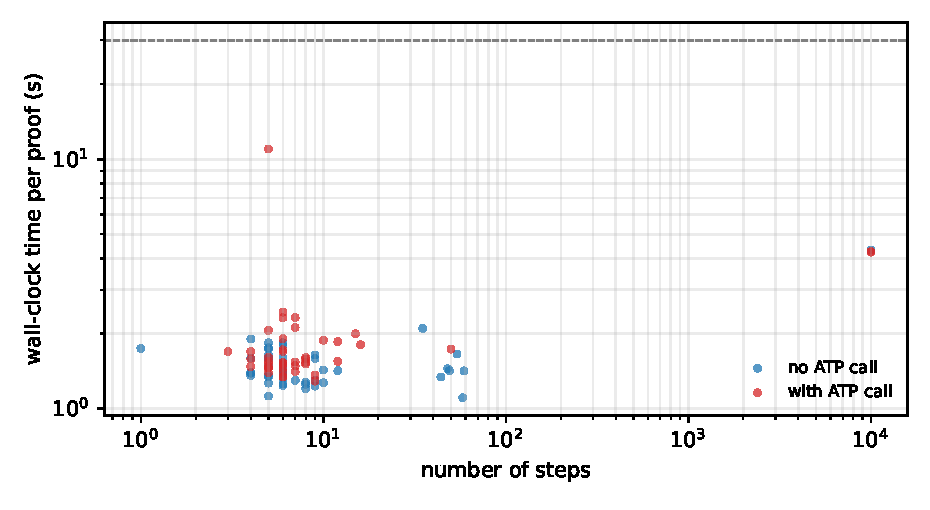
\includegraphics[width=\linewidth]{diagrams/runtime_scatter.pdf}
[Placeholder: wall-clock time per proof against the number of steps]
\caption{Wall-clock time per proof of the ProoVer set against the number of steps.}
\label{fig:eval-runtime}
\end{figure}

We also report where the time goes for the slowest proofs: parsing (LALR parser and transformer), global checks, rule checks, and ATP calls, and the peak memory of the worker process ([MB], measured with [tool]).
Deeply nested stress tests such as \texttt{PRV042} show whether the larger stack of Section~\ref{subsec:impl-resources} suffices: [result].

\subsection{Robustness (RQ3)}
\label{subsec:eval-robustness}

Robustness is evaluated in three ways.
First, the mutation test generates variants of valid seed proofs by applying one mutation each, such as changing a connective, swapping quantifiers, renaming a Skolem symbol to an existing one, or deleting a premise (Table~\ref{tab:eval-mutations}); a mutant is \emph{killed} if the verifier does not accept it.
Second, syntactically broken inputs (truncated files, unknown rules, missing annotations, deeply nested formulas) must neither crash the verifier nor lead to acceptance; we report the outcome for each class.
Third, we repeat the ProoVer run with the external prover removed from the path.
With the fail-closed policy, the number of wrong acceptances must stay at zero; the number of verified proofs drops by the proofs that need the ATP, and these proofs become uncertain.
This experiment verifies NFR1 empirically.

\begin{table}[t]
\centering
\small
\caption{Mutation operators and kill rates.}
\label{tab:eval-mutations}
\begin{tabular}{@{}l r r r@{}}
\toprule
Mutation operator & Mutants & Killed & Kill rate \\
\midrule
Change connective & [ ] & [ ] & [ ]\,\% \\
Swap quantifier kind & [ ] & [ ] & [ ]\,\% \\
Reuse existing symbol as Skolem symbol & [ ] & [ ] & [ ]\,\% \\
Remove premise & [ ] & [ ] & [ ]\,\% \\
\dots & & & \\
\midrule
Total & [ ] & [ ] & [ ]\,\% \\
\bottomrule
\end{tabular}
\end{table}

\subsection{Ablations}
\label{subsec:eval-ablation}

Two ablations quantify the design decisions of Table~\ref{tab:design-decisions}.
\emph{Syntactic checks first:} we run the verifier with all rule checkers disabled, so that every step goes to the external prover, and compare score and run time.
This shows what the internal checkers buy: [time factor] and [difference in score].
\emph{Three-valued verdict:} we replace the verdict rule by a binary one, in which unresolved steps count as failures, and recompute the score; the difference [D] shows the value of abstaining as described in Section~\ref{subsec:req-scoring}.
% Optional: Parser-Ablation (LALR vs. Earley) nur, falls ein Earley-Baseline noch existiert.

\subsection{Error Analysis}
\label{subsec:eval-errors}

We classify every proof of the ProoVer set whose verdict differs from the best possible one (acceptance of a valid proof, rejection of an invalid one) by its cause.
Table~\ref{tab:eval-errors} counts them by category: unsupported or imprecisely checked rule, missing ATP result, timeout, parser limitation, and expected result uncertain.
% TODO: pro Kategorie 1--2 konkrete Beispiele (Schrittname, Regel, Grund); bei Rewrite explizit auf die bekannte Lücke eingehen (Discussion).

\begin{table}[t]
\centering
\small
\caption{Causes of suboptimal verdicts on the ProoVer set.}
\label{tab:eval-errors}
\begin{tabular}{@{}l r l@{}}
\toprule
Cause & Proofs & Example \\
\midrule
Rule not checked precisely (e.g.\ \texttt{rewrite}) & [ ] & [ ] \\
ATP unresolved (timeout, no status) & [ ] & [ ] \\
Time limit exceeded & [ ] & [ ] \\
Parser or normalization limitation & [ ] & [ ] \\
\bottomrule
\end{tabular}
\end{table}

\subsection{Threats to Validity}
\label{subsec:eval-threats}

\paragraph{Internal validity.}
The verifier was developed against the ProoVer 2026 sample proofs, so the ProoVer set is not an independent test set; the TST set was written by the author and reflects the author's understanding of the rules.
The expected results of the ProoVer set depend on [source].
We mitigate this by reporting the mutation experiments, which do not depend on the benchmark, and by separating the wrong acceptances from the other errors.

\paragraph{External validity.}
The benchmark contains FOF proofs from a fixed set of generators; the results do not transfer to proofs from other provers with different rule vocabularies or to other logics.
The scoring scheme and the 30\,s limit are those of one competition.

\paragraph{Construct validity.}
The correctness of the accepted proofs relies on the correctness of the rule checkers, which is supported by tests but not proved, and on the soundness of the external prover.
Run times depend on the hardware and on the prover version and are therefore reported with their environment and as medians over several runs.

\subsection{Summary}
\label{subsec:eval-summary}

[TODO: three to five sentences answering RQ1--RQ3 with the key numbers; the full answers follow in Chapter~\ref{sec:conclusion}.]
% Werte in [eckigen Klammern] nach der Evaluation eintragen. Absätze mit "% FALLS" je nach Stand des Codes beibehalten oder streichen.

\section{Discussion}
\label{sec:discussion}

This chapter interprets the results of Chapter~\ref{sec:evaluation}, discusses what the verifier does and does not guarantee, and lists its limitations.

\subsection{Interpretation of the Results}
\label{subsec:disc-results}

The verifier reaches a score of [S] of 153 points on the ProoVer set and does not accept any invalid proof [confirm].
The second property matters more than the first: with a penalty of $-10$ for a wrong acceptance, a single such error costs as much as ten correct acceptances.
The verdict matrix shows where the remaining points are lost.
[Interpretation: most losses are abstentions on valid proofs, caused by [rule / timeout / ATP], and not wrong rejections.]
This is the intended behavior of the fail-closed policy of Section~\ref{subsec:req-scoring}: when the verifier loses points, it loses them in the cheap direction.

The ablation of the verdict rule (Section~\ref{subsec:eval-ablation}) quantifies this: a binary verdict that treats unresolved steps as failures would have changed the score by [D] points, because [it turns abstentions on invalid proofs into lucky rejections but also turns abstentions on valid proofs into wrong rejections].
The comparison also shows that the benefit of abstaining depends on the benchmark: it pays off when unresolved steps are rare but dangerous, and it is worth little when almost every proof can be decided.

The rule coverage (Section~\ref{subsec:eval-coverage}) shows that [X\,\%] of the steps are decided by internal checks, and only [Y\,\%] need the external prover.
At the same time, the run times (Section~\ref{subsec:eval-runtime}) are dominated by the ATP calls: a single call takes about two seconds in our preliminary measurements, while all internal checks of a proof together take [milliseconds to a few hundred milliseconds].
For this reason, the order ``cheap checks first'' is not only a design preference but the main lever for the run time, and it is the reason why the verifier stays within the 30\,s limit on [Z] of the proofs.

\subsection{Scoring Policy and Its Limits}
\label{subsec:disc-scoring}

The policy of Section~\ref{subsec:req-scoring} follows from the scoring scheme, but it rests on assumptions that deserve a comment.
The probability $p$ that a proof is valid is not observable, so the thresholds $2/3$ and $10/11$ cannot be applied literally; the verifier approximates them by the discrete rule that acceptance requires positive evidence for every step and rejection requires a concrete defect.
This is conservative on both sides.
It would be possible to accept proofs with a small unresolved remainder if the remainder is judged harmless, but this requires a calibrated estimate of $p$ that the verifier does not have.
The policy is also tied to this competition: with a different penalty the optimal behavior changes, and in a setting where a wrong acceptance is not much worse than a wrong rejection, abstention would be less attractive.
Finally, the policy trades points for safety when the external prover is missing or too slow: invalid proofs whose defect is only visible to the prover become \emph{uncertain} instead of being rejected, and the verifier forgoes the $+2$ for them.

\subsection{Trusted Computing Base and Soundness}
\label{subsec:disc-tcb}

The soundness argument of Section~\ref{subsec:design-verdict} is conditional: it holds if the rule checkers are correct and the external prover is sound.
In terms of the trusted computing base (Section~\ref{subsec:atp-certification}), the following components therefore have to be trusted for the property that every accepted proof is valid:
\begin{itemize}
  \item the \emph{parser and normalization}, since a parse error that changes the meaning of a formula would change what is checked;
  \item the \emph{alpha-equivalence} check, which also merges quantifier prefixes and flattens junctions before it compares, and which therefore equates formulas that are not literally identical;
  \item the \emph{rule checkers}, in particular the Skolem checker, the largest module, and the clausal checker;
  \item the \emph{serialization of formulas to TPTP} for the external prover, because a defect there would make the prover validate a different formula than the one in the proof;
  \item the \emph{external prover} and its interpretation through the SZS status line; and
  \item the \emph{verdict aggregation}, which decides how the individual results are combined.
\end{itemize}
Compared with a checker that sends every step to a prover, this list is longer, because the internal checks are part of it; compared with the prover that produced the proof, it is much shorter.
This is the trade-off stated in Section~\ref{subsec:rw-positioning}: the thesis exchanges a larger trusted checker for less dependence on the prover and for better diagnostics.
The evaluation supports the correctness of the checkers by tests, by the mutation experiment, and by the benchmark, but it does not prove it.
A way to reduce the trusted part further would be to restrict the internal checks to the rules where they are simple (structural, propositional, and the Skolem conditions) and to delegate the rest, or to validate the checks themselves against a proof assistant.

\subsection{Design Trade-offs}
\label{subsec:disc-tradeoffs}

\paragraph{Internal checks and ATP fallback.}
The competition rules allow any step except Skolemization and the import steps to be checked by an external prover.
A single step that derives \texttt{\$false} directly from the axioms and the negated conjecture is then delegated completely (the test group \texttt{st08} contains such a ``monolithic'' step).
For such proofs the verifier is exactly as strong as the prover, and the internal checks contribute only the global conditions.
This is correct with respect to the rules, but it shows that the quality of the verifier on such inputs lies in the global checks, not in the step checks.

\paragraph{Modularity.}
Rule-local checkers made it possible to test each rule in isolation and to attribute every error to a step and a reason.
The price is that some knowledge, such as the freshness of Skolem symbols, cannot be local to one step and lives in the driver.
The size of the dispatcher in \texttt{main.py} is a sign that the modular idea has been applied to the checkers but not yet to the dispatch; the registry of Section~\ref{subsec:design-dispatch} addresses this.

\paragraph{Python.}
The implementation language favors readability and fast development, which was valuable for a thesis with many rules.
It costs run time for the internal checks and complicates deep recursion, which needed a dedicated thread with a larger stack.
The measurements show that the ATP, not Python, dominates the run time of the proofs that need it; the pure Python cost matters for the large proofs, where [parsing / checks] take [x\,s].

\paragraph{Process isolation.}
Running each proof in its own process makes timeouts and crashes harmless and enforces the time limit, but it adds a startup cost per proof and makes sharing state, such as a cache of ATP results, harder.

\subsection{Limitations}
\label{subsec:disc-limitations}

\begin{itemize}
  \item \textbf{Logic and format.} The verifier handles FOF problems and TSTP proofs with the rule vocabulary of the ProoVer 2026 benchmarks. CNF, typed, and higher-order input are out of scope, and rules outside the supported set are delegated to the prover or lead to abstention.
  \item \textbf{Weak rule checks.} The \texttt{rewrite} rule is checked only for the shapes observed in the benchmark, because the demodulating equation may be missing in the proof. Since this check is weaker than the logical meaning of the rule, an accepted \texttt{rewrite} step is less well justified than the other steps. % FALLS rewrite an den ATP delegiert bzw. unresolved wird: diesen Punkt streichen.
  \item \textbf{Symbols from instantiation.} Annotations of Herbrand symbols are parsed but not checked separately. This is sound for \texttt{thm} steps, since instantiation with an arbitrary term is entailed by the parent, but it means that the annotation carries no checked information. % FALLS im Code behandelt: anpassen.
  \item \textbf{Sequential prover calls.} Each unresolved step starts its own prover process, one after another. Proofs with many such steps are therefore slow. Parallel calls and a shared time budget would help.
  \item \textbf{Benchmark.} The ProoVer set contains 100 proofs and the TST set 76 proofs written by the author. This is enough to find defects, but not to estimate rare failure rates, and the results do not carry over to proofs from other provers (Section~\ref{subsec:eval-threats}).
  \item \textbf{Trust in tests.} Correctness of the checkers is supported by tests and mutations, not proved.
\end{itemize}
\section{Conclusion and Future Work}
\label{sec:conclusion}

\subsection{Summary}

This thesis designed and implemented a Python-based verifier for TSTP derivations for the ProoVer 2026 competition.
The starting point was the observation that the competition's scoring scheme is highly asymmetric: a wrongly accepted proof costs ten points, a correct acceptance gains one.
From the expected score of the three possible answers, we derived a fail-closed policy with a three-valued verdict: the verifier accepts only if every step is validated positively, rejects only if it has found a concrete defect, and abstains otherwise.
The verifier realizes this policy as a modular pipeline: a parser, global checks of provenance, dependencies, and the negated conjecture, rule-local checkers for structural, propositional, quantifier, and clausal rules, a dedicated check for Skolemization including the freshness of the introduced symbols, and a restricted fallback to an external prover for the remaining steps.
A soundness argument shows that acceptance implies unsatisfiability of the axioms together with the negated conjecture, under the assumption that the rule checkers are correct and the prover is sound.

\subsection{Answers to the Research Questions}

\paragraph{RQ1: Which rules and fragments must be supported?}
The ProoVer 2026 benchmarks use [N] distinct inference rules.
Of these, [A] are checked internally, which covers [X\,\%] of all steps; the remaining [B] rules, among them \texttt{consequence}, are delegated to the prover.
Skolemization is the one rule that has to be checked internally, since it preserves only satisfiability and cannot be validated by entailment, and the checks for quantifier scope, polarity, and freshness are needed to reject the subtle errors in the invalid proofs.

\paragraph{RQ2: How does modularity keep the trusted part small and extensible?}
Every rule check is a function of a step and its parents and returns structured issues.
The checkers can be tested in isolation, which is reflected in a test suite of about 250 tests with a coverage of [C\,\%], and an error can be attributed to a step and a reason.
The trusted part consists of the parser, the alpha-equivalence check, the rule checkers, the serialization to the prover, and the verdict aggregation, in total about [L] lines, plus the external prover as an assumption (Section~\ref{subsec:disc-tcb}).
[Extending the verifier by a rule required [k] lines in [m] files.]

\paragraph{RQ3: How do correctness, run time, and memory behave?}
On the ProoVer set, the verifier reaches [S] of 153 points with [W] wrong acceptances, a median run time of [t\,s], and a maximum of [t$_{\max}$\,s]; [T] proofs hit the time limit.
The mutation experiment kills [M\,\%] of [N] mutants, and with the prover removed the verifier still makes no wrong acceptance, which confirms the fail-closed property empirically.
Run time is dominated by the calls to the external prover, not by the internal checks.

\subsection{Contributions Revisited}

The thesis contributes (i) a verdict policy for proof checking derived from the scoring scheme, together with a soundness argument that accounts for the different semantics of \texttt{thm} and \texttt{esa} steps; (ii) a modular architecture and its implementation with a dedicated Skolem check and a restricted ATP fallback; and (iii) an evaluation on the competition benchmark and on a suite of mutated and hand-written proofs that measures correctness, coverage, run time, and robustness, with an analysis of the remaining limitations.

\subsection{Future Work}

Several directions follow from the limitations of Section~\ref{subsec:disc-limitations}.
\begin{itemize}
  \item \textbf{Registry-based dispatch.} Replace the \texttt{if}/\texttt{elif} dispatcher by the registry of the design, so that adding a rule needs one entry and one function.
  \item \textbf{Stronger checks for weak rules.} Reconstruct the missing demodulating equation of \texttt{rewrite} steps, or validate them against a prover, and add checks for Herbrand symbols once their meaning is fixed by the specification.
  \item \textbf{Counter-model search.} Use a model finder to reject steps that are not entailed, as N\"orgler does, which would turn more unresolved steps into defects and thereby recover the $+2$ for invalid proofs.
  \item \textbf{Parallel and budgeted prover calls.} Run the prover calls for independent steps in parallel under a shared time budget, and cache results across steps.
  \item \textbf{Smaller trusted base.} Validate the internal checks themselves, for example by formalizing the Skolem conditions in a proof assistant, or produce certificates that a small kernel can check, following the approaches discussed in Chapter~\ref{sec:related-work}.
  \item \textbf{Broader input.} Support CNF proofs and further rule vocabularies, and compare the verifier with GDV and N\"orgler on a common benchmark.
\end{itemize}

\appendix

\section{Reproduction}
\label{app:reproduction}

This appendix describes how to reproduce the results of the thesis.
The source code, the proofs, and the scripts are in the repository of the thesis; the commit used for the measurements is \EvalCommit.

\subsection{Requirements}

The verifier needs Python~3.11 or newer (the measurements used Python~\EvalPython) and the library \texttt{lark}.
The external prover is Vampire (the measurements used \EvalVampire).
Vampire is called through the environment variables \texttt{EXTERNAL\_ATP\_BINARY} (path of the binary) or \texttt{EXTERNAL\_ATP\_COMMAND} (complete command), and is found in the search path by default.
Under Windows, the verifier is run in WSL.

\begin{verbatim}
python3 -m venv .venv && source .venv/bin/activate
python -m pip install -r requirements.txt -r requirements-dev.txt
export EXTERNAL_ATP_BINARY=/usr/local/bin/vampire
\end{verbatim}

\subsection{Checking Proofs}

A single proof is checked by passing the proof file; the problem file is looked up in the subdirectory \texttt{Problems} next to the proof, or given with \texttt{-p}.
Without a proof argument, the verifier checks all proofs of a directory (default \texttt{ProoVer2026/PRV}; further sets are \texttt{ProoVer2026/Test}, \texttt{ProoVer2026/Extra}, and \texttt{ProoVer2026/Deprecated}) and prints a summary with the score.

\begin{verbatim}
python main.py ProoVer2026/PRV/PRV010+1.s
python main.py proof.s -p problem.p -t 30
python main.py -d ProoVer2026/Extra
python main.py --binary-verdict ProoVer2026/PRV/PRV010+1.s
\end{verbatim}

\begin{table}[tbp]
\centering
\small
\caption{Command-line options of the verifier.}
\label{tab:app-cli}
\begin{tabular}{@{}l P{0.65\linewidth}@{}}
\toprule
Option & Meaning \\
\midrule
\texttt{-p}, \texttt{--problem} & Problem file; by default \texttt{Problems/<name>.p} next to the proof. \\
\texttt{-t}, \texttt{--timeout} & Wall-clock limit per proof in seconds (default 30). \\
\texttt{-d}, \texttt{--dir} & Batch mode: directory with proofs; the expected results are chosen from the directory name (\texttt{-e} overrides). \\
\texttt{--prefix} & Batch mode: only check proofs whose file name starts with the prefix. \\
\texttt{--binary-verdict} & Print \texttt{VerifiedBad} instead of \texttt{Unknown} when a step cannot be decided. \\
\bottomrule
\end{tabular}
\end{table}

The last line of the output is the SZS status.
Table~\ref{tab:app-status} lists the statuses.

\begin{table}[tbp]
\centering
\small
\caption{Statuses printed by the verifier.}
\label{tab:app-status}
\begin{tabular}{@{}l P{0.65\linewidth}@{}}
\toprule
Status & Meaning \\
\midrule
\texttt{VerifiedGood} & Every check succeeded. \\
\texttt{VerifiedBad} & A definite defect was found, or the proof could not be processed. \\
\texttt{Unknown} & No defect was found, but a step could not be decided (prover without result, or no checker for the rule). \\
\texttt{Timeout} & The time limit was exceeded. \\
\bottomrule
\end{tabular}
\end{table}

\subsection{Tests and Evaluation}

The test suite is run with \texttt{pytest}; the coverage figures of Section~\ref{subsec:eval-modularity} come from the same run.
The evaluation driver runs the verifier in a fresh process for each proof and writes raw data to \texttt{results/eval} and the tables and macros of Chapter~\ref{sec:evaluation} to \texttt{thesis/generated}.

\begin{verbatim}
pytest
python scripts/eval_all.py --parts all --reps 3
python scripts/gen_appendix_tables.py
\end{verbatim}

\noindent The parts of the driver can be run separately with \texttt{--parts}; Table~\ref{tab:app-parts} lists them.
The run time depends on the machine; the full run needs the prover for all parts except \texttt{noatp}.

\begin{table}[tbp]
\centering
\small
\caption{Parts of the evaluation driver \texttt{scripts/eval\_all.py}.}
\label{tab:app-parts}
\begin{tabular}{@{}l P{0.70\linewidth}@{}}
\toprule
Part & Content \\
\midrule
\texttt{runs} & Verdicts, steps, prover calls, time, and memory per proof (Sections~\ref{subsec:eval-correctness} and~\ref{subsec:eval-runtime}). \\
\texttt{noatp} & The same without prover (ablation). \\
\texttt{internal} & Internal checkers against Vampire on single steps. \\
\texttt{mutation} & Mutations of accepted proofs with entailment check of the survivors. \\
\texttt{inputs} & Malformed inputs (robustness). \\
\texttt{extra} & Generated rule test suite. \\
\texttt{coverage} & Test coverage and lines of code per module. \\
\texttt{tables} & Regenerates tables, macros, and the figures from the raw data. \\
\bottomrule
\end{tabular}
\end{table}

\section{Example Reports}
\label{app:reports}

The report lists one block per check, and ends with the SZS status.
The following output is the (shortened) report for the invalid proof \texttt{PRV002+1}, in which the negated conjecture is not the negation of the conjecture; the blocks without finding are omitted and the formulas are abbreviated.

\begin{verbatim}
Checking proof: ProoVer2026/PRV/PRV002+1.s
Against problem: ProoVer2026/PRV/Problems/PRV002+1.p

[FAIL] Negated Conjecture Issues:
  - neg: formula is not the correct negation of parent
    conjecture; expected one of: [...], got: [...]

% SZS status VerifiedBad
\end{verbatim}

\section{Results per Proof}
\label{app:per-proof}

Tables~\ref{tab:app-prv}, \ref{tab:app-tst}, and~\ref{tab:app-ext} list the status and the run time of each proof of the three benchmark groups.
The time is the median over the repetitions of the whole process, including the start-up of the interpreter.
The column ``Result'' compares the status with the expected result; ``abstain'' denotes \texttt{Unknown} or \texttt{Timeout}, which score zero.

{\small
\begin{longtable}{@{}l l l l r r@{}}
\caption{Results for each proof of the ProoVer set (official proofs and samples).}\label{tab:app-prv}\\
\toprule
Proof & Expected & Status & Result & Time (s) & ATP calls \\
\midrule
\endfirsthead
\toprule
Proof & Expected & Status & Result & Time (s) & ATP calls \\
\midrule
\endhead
\bottomrule
\endlastfoot
\texttt{PRV000{+}1} & correct & VerifiedGood & ok & 1.69 & 1 \\
\texttt{PRV001{+}1} & correct & VerifiedGood & ok & 1.39 & 0 \\
\texttt{PRV002{+}1} & incorrect & VerifiedBad & ok & 1.58 & 1 \\
\texttt{PRV003{+}1} & incorrect & VerifiedBad & ok & 1.47 & 1 \\
\texttt{PRV004{+}1} & correct & VerifiedGood & ok & 1.40 & 1 \\
\texttt{PRV005{+}1} & correct & VerifiedGood & ok & 1.85 & 1 \\
\texttt{PRV006{+}1} & incorrect & VerifiedBad & ok & 1.66 & 1 \\
\texttt{PRV007{+}1} & incorrect & VerifiedBad & ok & 1.30 & 0 \\
\texttt{PRV008{+}1} & incorrect & VerifiedBad & ok & 1.27 & 0 \\
\texttt{PRV009{+}1} & incorrect & VerifiedBad & ok & 1.45 & 1 \\
\texttt{PRV010{+}1} & correct & VerifiedGood & ok & 1.42 & 0 \\
\texttt{PRV011{+}1} & correct & VerifiedGood & ok & 1.66 & 0 \\
\texttt{PRV012{+}1} & correct & VerifiedGood & ok & 1.44 & 0 \\
\texttt{PRV013{+}1} & correct & VerifiedGood & ok & 1.42 & 0 \\
\texttt{PRV014{+}1} & correct & VerifiedGood & ok & 1.73 & 1 \\
\texttt{PRV015{+}1} & correct & VerifiedGood & ok & 1.34 & 0 \\
\texttt{PRV016{+}1} & correct & VerifiedGood & ok & 1.10 & 0 \\
\texttt{PRV017{+}1} & correct & VerifiedGood & ok & 1.55 & 2 \\
\texttt{PRV018{+}1} & correct & VerifiedGood & ok & 1.42 & 0 \\
\texttt{PRV019{+}1} & correct & VerifiedGood & ok & 1.36 & 1 \\
\texttt{PRV020{+}1} & correct & VerifiedGood & ok & 1.23 & 0 \\
\texttt{PRV021{+}1} & correct & VerifiedGood & ok & 1.20 & 0 \\
\texttt{PRV022{+}1} & correct & VerifiedGood & ok & 1.29 & 2 \\
\texttt{PRV023{+}1} & incorrect & VerifiedBad & ok & 1.26 & 0 \\
\texttt{PRV024{+}1} & incorrect & VerifiedBad & ok & 1.28 & 0 \\
\texttt{PRV025{+}1} & incorrect & VerifiedBad & ok & 1.74 & 0 \\
\texttt{PRV026{+}1} & incorrect & VerifiedBad & ok & 2.12 & 1 \\
\texttt{PRV027{+}1} & correct & VerifiedGood & ok & 1.59 & 0 \\
\texttt{PRV028{+}1} & incorrect & VerifiedBad & ok & 1.53 & 1 \\
\texttt{PRV029{+}1} & correct & VerifiedGood & ok & 1.30 & 0 \\
\texttt{PRV030{+}1} & correct & VerifiedGood & ok & 1.34 & 1 \\
\texttt{PRV031{+}1} & incorrect & VerifiedBad & ok & 1.47 & 1 \\
\texttt{PRV032{+}1} & incorrect & VerifiedBad & ok & 1.24 & 0 \\
\texttt{PRV033{+}1} & correct & VerifiedGood & ok & 1.25 & 0 \\
\texttt{PRV034{+}1} & correct & VerifiedGood & ok & 1.43 & 0 \\
\texttt{PRV035{+}1} & incorrect & VerifiedBad & ok & 1.59 & 0 \\
\texttt{PRV036{+}1} & incorrect & VerifiedBad & ok & 1.42 & 0 \\
\texttt{PRV037{+}1} & incorrect & VerifiedBad & ok & 1.39 & 0 \\
\texttt{PRV038{+}1} & incorrect & VerifiedBad & ok & 1.34 & 1 \\
\texttt{PRV039{+}1} & incorrect & VerifiedBad & ok & 1.36 & 0 \\
\texttt{PRV040{+}1} & correct & VerifiedGood & ok & 1.41 & 1 \\
\texttt{PRV041{+}1} & correct & VerifiedGood & ok & 1.33 & 0 \\
\texttt{PRV042{+}1} & correct & VerifiedGood & ok & 1.69 & 1 \\
\texttt{PRV043{+}1} & correct & VerifiedGood & ok & 2.06 & 1 \\
\texttt{PRV044{+}1} & correct & VerifiedGood & ok & 1.90 & 1 \\
\texttt{PRV045{+}1} & correct & VerifiedGood & ok & 1.26 & 0 \\
\texttt{PRV046{+}1} & incorrect & VerifiedBad & ok & 1.42 & 0 \\
\texttt{PRV047{+}1} & incorrect & VerifiedBad & ok & 1.12 & 0 \\
\texttt{PRV048{+}1} & correct & VerifiedGood & ok & 1.34 & 0 \\
\texttt{PRV049{+}1} & incorrect & VerifiedBad & ok & 1.63 & 0 \\
\texttt{PRV050{+}1} & incorrect & VerifiedBad & ok & 1.84 & 0 \\
\texttt{PRV051{+}1} & incorrect & VerifiedBad & ok & 1.75 & 0 \\
\texttt{PRV052{+}1} & incorrect & VerifiedBad & ok & 1.59 & 0 \\
\texttt{PRV053{+}1} & incorrect & VerifiedBad & ok & 1.36 & 0 \\
\texttt{PRV054{+}1} & incorrect & VerifiedBad & ok & 1.50 & 0 \\
\texttt{PRV055{+}1} & correct & VerifiedGood & ok & 1.59 & 0 \\
\texttt{PRV056{+}1} & incorrect & VerifiedBad & ok & 1.70 & 1 \\
\texttt{PRV057{+}1} & incorrect & Error & ok & 1.89 & 0 \\
\texttt{PRV058{+}1} & incorrect & VerifiedBad & ok & 1.60 & 1 \\
\texttt{PRV059{+}1} & correct & VerifiedGood & ok & 1.53 & 1 \\
\texttt{PRV060{+}1} & correct & VerifiedGood & ok & 1.58 & 1 \\
\texttt{PRV061{+}1} & correct & VerifiedGood & ok & 1.86 & 3 \\
\texttt{PRV062{+}1} & correct & VerifiedGood & ok & 1.88 & 2 \\
\texttt{PRV063{+}1} & correct & VerifiedGood & ok & 2.00 & 1 \\
\texttt{PRV064{+}1} & correct & VerifiedGood & ok & 1.80 & 4 \\
\texttt{PRV065{+}1} & incorrect & VerifiedBad & ok & 1.77 & 1 \\
\texttt{PRV066{+}1} & incorrect & VerifiedBad & ok & 1.72 & 1 \\
\texttt{PRV067{+}1} & incorrect & VerifiedBad & ok & 1.38 & 0 \\
\texttt{PRV068{+}1} & incorrect & VerifiedBad & ok & 1.48 & 0 \\
\texttt{PRV069{+}1} & incorrect & VerifiedBad & ok & 1.52 & 1 \\
\texttt{PRV070{+}1} & correct & VerifiedGood & ok & 1.40 & 0 \\
\texttt{PRV071{+}1} & incorrect & VerifiedBad & ok & 4.24 & 1 \\
\texttt{PRV072{+}1} & incorrect & VerifiedBad & ok & 4.33 & 0 \\
\texttt{PRV073{+}1} & correct & VerifiedGood & ok & 4.27 & 1 \\
\texttt{PRV074{+}1} & incorrect & VerifiedBad & ok & 1.49 & 1 \\
\texttt{PRV075{+}1} & incorrect & VerifiedBad & ok & 1.51 & 1 \\
\texttt{PRV076{+}1} & correct & VerifiedGood & ok & 1.54 & 2 \\
\texttt{PRV077{+}1} & incorrect & VerifiedBad & ok & 1.41 & 1 \\
\texttt{PRV078{+}1} & incorrect & VerifiedBad & ok & 1.50 & 1 \\
\texttt{PRV079{+}1} & correct & VerifiedGood & ok & 1.62 & 1 \\
\texttt{PRV080{+}1} & incorrect & VerifiedBad & ok & 1.69 & 1 \\
\texttt{PRV081{+}1} & correct & VerifiedGood & ok & 1.61 & 1 \\
\texttt{PRV082{+}1} & correct & VerifiedGood & ok & 1.46 & 1 \\
\texttt{PRV083{+}1} & incorrect & VerifiedBad & ok & 1.41 & 0 \\
\texttt{PRV084{+}1} & incorrect & VerifiedBad & ok & 1.53 & 1 \\
\texttt{PRV085{+}1} & correct & VerifiedGood & ok & 1.54 & 1 \\
\texttt{PRV086{+}1} & incorrect & VerifiedBad & ok & 1.45 & 1 \\
\texttt{PRV087{+}1} & incorrect & VerifiedBad & ok & 1.72 & 1 \\
\texttt{PRV088{+}1} & correct & VerifiedGood & ok & 1.91 & 1 \\
\texttt{PRV089{+}1} & correct & VerifiedGood & ok & 1.59 & 0 \\
\texttt{PRV090{+}1} & incorrect & VerifiedBad & ok & 1.64 & 0 \\
\texttt{PRV091{+}1} & incorrect & Error & ok & 1.74 & 0 \\
\texttt{PRV092{+}1} & incorrect & VerifiedBad & ok & 2.32 & 1 \\
\texttt{PRV093{+}1} & incorrect & VerifiedBad & ok & 2.44 & 1 \\
\texttt{PRV094{+}1} & incorrect & VerifiedBad & ok & 2.31 & 1 \\
\texttt{PRV095{+}1} & incorrect & VerifiedBad & ok & 1.84 & 0 \\
\texttt{PRV096{+}1} & correct & VerifiedGood & ok & 1.79 & 0 \\
\texttt{PRV097{+}1} & incorrect & Unknown & abstain & 1.90 & 0 \\
\texttt{PRV098{+}1} & correct & VerifiedGood & ok & 2.10 & 0 \\
\texttt{PRV099{+}1} & incorrect & VerifiedBad & ok & 11.00 & 2 \\
\end{longtable}

}

{\small
\begin{longtable}{@{}l l l l r r@{}}
\caption{Results for each proof of the TST set (own test proofs).}\label{tab:app-tst}\\
\toprule
Proof & Expected & Status & Result & Time (s) & ATP calls \\
\midrule
\endfirsthead
\toprule
Proof & Expected & Status & Result & Time (s) & ATP calls \\
\midrule
\endhead
\bottomrule
\endlastfoot
\texttt{TST001{+}1} & correct & VerifiedGood & ok & 1.19 & 0 \\
\texttt{TST002{+}1} & correct & VerifiedGood & ok & 1.22 & 0 \\
\texttt{TST003{+}1} & correct & VerifiedGood & ok & 1.28 & 0 \\
\texttt{TST004{+}1} & correct & VerifiedGood & ok & 1.24 & 0 \\
\texttt{TST005{+}1} & correct & VerifiedGood & ok & 1.30 & 0 \\
\texttt{TST006{+}1} & correct & VerifiedGood & ok & 1.27 & 0 \\
\texttt{TST007{+}1} & correct & VerifiedGood & ok & 1.37 & 0 \\
\texttt{TST008{+}1} & incorrect & VerifiedBad & ok & 1.61 & 0 \\
\texttt{TST009{+}1} & incorrect & VerifiedBad & ok & 1.57 & 0 \\
\texttt{TST010{+}1} & incorrect & VerifiedBad & ok & 1.24 & 0 \\
\texttt{TST011{+}1} & incorrect & VerifiedBad & ok & 1.29 & 0 \\
\texttt{TST012{+}1} & incorrect & VerifiedBad & ok & 1.21 & 0 \\
\texttt{TST013{+}1} & incorrect & VerifiedBad & ok & 1.18 & 0 \\
\texttt{TST014{+}1} & incorrect & VerifiedBad & ok & 1.22 & 0 \\
\texttt{TST015{+}1} & incorrect & VerifiedBad & ok & 1.30 & 0 \\
\texttt{TST016{+}1} & incorrect & VerifiedBad & ok & 1.41 & 0 \\
\texttt{TST017{+}1} & incorrect & VerifiedBad & ok & 1.19 & 0 \\
\texttt{TST018{+}1} & incorrect & VerifiedBad & ok & 1.28 & 0 \\
\texttt{TST019{+}1} & incorrect & VerifiedBad & ok & 1.15 & 0 \\
\texttt{TST020{+}1} & incorrect & Unknown & abstain & 1.18 & 0 \\
\texttt{TST021{+}1} & incorrect & VerifiedBad & ok & 1.24 & 0 \\
\texttt{TST022{+}1} & incorrect & VerifiedBad & ok & 1.28 & 0 \\
\texttt{TST023{+}1} & incorrect & VerifiedBad & ok & 1.75 & 1 \\
\texttt{TST024{+}1} & incorrect & VerifiedBad & ok & 1.65 & 1 \\
\texttt{TST025{+}1} & incorrect & VerifiedBad & ok & 1.33 & 0 \\
\texttt{TST026{+}1} & incorrect & VerifiedBad & ok & 1.46 & 1 \\
\texttt{TST027{+}1} & incorrect & VerifiedBad & ok & 1.24 & 0 \\
\texttt{TST028{+}1} & incorrect & VerifiedBad & ok & 1.28 & 0 \\
\texttt{TST029{+}1} & incorrect & VerifiedBad & ok & 1.26 & 0 \\
\texttt{TST030{+}1} & incorrect & VerifiedBad & ok & 1.36 & 0 \\
\texttt{TST031{+}1} & incorrect & VerifiedBad & ok & 1.40 & 0 \\
\texttt{TST032{+}1} & incorrect & VerifiedBad & ok & 1.30 & 0 \\
\texttt{TST033{+}1} & incorrect & VerifiedBad & ok & 1.32 & 0 \\
\texttt{TST034{+}1} & incorrect & VerifiedBad & ok & 1.28 & 0 \\
\texttt{TST035{+}1} & incorrect & VerifiedBad & ok & 1.27 & 0 \\
\texttt{TST036{+}1} & incorrect & VerifiedBad & ok & 1.33 & 0 \\
\texttt{TST037{+}1} & incorrect & VerifiedBad & ok & 1.49 & 1 \\
\texttt{TST038{+}1} & incorrect & VerifiedBad & ok & 1.56 & 0 \\
\texttt{TST039{+}1} & incorrect & VerifiedBad & ok & 1.25 & 0 \\
\texttt{TST040{+}1} & incorrect & Error & ok & 1.24 & 0 \\
\texttt{TST041{+}1} & incorrect & VerifiedBad & ok & 1.29 & 0 \\
\texttt{TST042{+}1} & incorrect & VerifiedBad & ok & 1.21 & 0 \\
\texttt{TST043{+}1} & incorrect & VerifiedGood & wrong accept & 1.23 & 1 \\
\texttt{TST044{+}1} & incorrect & VerifiedBad & ok & 1.30 & 0 \\
\texttt{TST045{+}1} & incorrect & VerifiedBad & ok & 1.33 & 0 \\
\texttt{TST046{+}1} & incorrect & VerifiedBad & ok & 1.26 & 0 \\
\texttt{TST047{+}1} & correct & VerifiedGood & ok & 1.23 & 0 \\
\texttt{TST048{+}1} & correct & VerifiedGood & ok & 1.29 & 0 \\
\texttt{TST049{+}1} & correct & VerifiedGood & ok & 1.26 & 0 \\
\texttt{TST050{+}1} & correct & VerifiedGood & ok & 1.19 & 0 \\
\texttt{TST051{+}1} & correct & VerifiedGood & ok & 1.28 & 0 \\
\texttt{TST052{+}1} & correct & VerifiedGood & ok & 1.57 & 1 \\
\texttt{TST053{+}1} & incorrect & VerifiedBad & ok & 1.55 & 0 \\
\texttt{TST054{+}1} & incorrect & VerifiedBad & ok & 1.34 & 0 \\
\texttt{TST055{+}1} & incorrect & VerifiedBad & ok & 1.28 & 0 \\
\texttt{TST056{+}1} & incorrect & VerifiedBad & ok & 1.21 & 0 \\
\texttt{TST057{+}1} & incorrect & VerifiedBad & ok & 1.22 & 0 \\
\texttt{TST058{+}1} & incorrect & VerifiedBad & ok & 1.21 & 0 \\
\texttt{TST059{+}1} & incorrect & VerifiedBad & ok & 1.38 & 0 \\
\texttt{TST060{+}1} & incorrect & VerifiedBad & ok & 1.23 & 0 \\
\texttt{TST061{+}1} & incorrect & VerifiedBad & ok & 1.27 & 0 \\
\texttt{TST062{+}1} & incorrect & VerifiedBad & ok & 1.21 & 0 \\
\texttt{TST063{+}1} & incorrect & VerifiedBad & ok & 1.25 & 0 \\
\texttt{TST064{+}1} & incorrect & VerifiedBad & ok & 1.56 & 0 \\
\texttt{TST065{+}1} & incorrect & VerifiedBad & ok & 1.29 & 1 \\
\texttt{TST066{+}1} & incorrect & VerifiedBad & ok & 1.07 & 0 \\
\texttt{TST067{+}1} & incorrect & VerifiedBad & ok & 1.21 & 0 \\
\texttt{TST068{+}1} & edge & VerifiedGood & edge case & 1.39 & 0 \\
\texttt{TST069{+}1} & incorrect & VerifiedBad & ok & 1.22 & 0 \\
\texttt{TST070{+}1} & incorrect & VerifiedBad & ok & 1.28 & 0 \\
\texttt{TST071{+}1} & edge & VerifiedGood & edge case & 1.26 & 0 \\
\texttt{TST072{+}1} & incorrect & VerifiedBad & ok & 1.25 & 0 \\
\texttt{TST073{+}1} & edge & VerifiedGood & edge case & 1.23 & 0 \\
\texttt{TST074{+}1} & edge & VerifiedBad & edge case & 1.31 & 0 \\
\texttt{TST075{+}1} & incorrect & VerifiedBad & ok & 1.36 & 1 \\
\texttt{TST076{+}1} & edge & VerifiedBad & edge case & 1.32 & 1 \\
\end{longtable}

}

{\small
\begin{longtable}{@{}l l l l r r@{}}
\caption{Results for each proof of the Extra set (generated rule-level test proofs).}\label{tab:app-ext}\\
\toprule
Proof & Expected & Status & Result & Time (s) & ATP calls \\
\midrule
\endfirsthead
\toprule
Proof & Expected & Status & Result & Time (s) & ATP calls \\
\midrule
\endhead
\bottomrule
\endlastfoot
\texttt{EXT001{+}1} & correct & VerifiedGood & ok & 1.28 & 0 \\
\texttt{EXT002{+}1} & incorrect & VerifiedBad & ok & 1.31 & 0 \\
\texttt{EXT003{+}1} & incorrect & VerifiedBad & ok & 1.20 & 0 \\
\texttt{EXT004{+}1} & incorrect & VerifiedBad & ok & 1.20 & 0 \\
\texttt{EXT005{+}1} & incorrect & VerifiedBad & ok & 1.33 & 0 \\
\texttt{EXT006{+}1} & incorrect & VerifiedBad & ok & 1.20 & 0 \\
\texttt{EXT007{+}1} & correct & VerifiedGood & ok & 1.24 & 0 \\
\texttt{EXT008{+}1} & incorrect & VerifiedBad & ok & 1.50 & 0 \\
\texttt{EXT009{+}1} & edge & VerifiedBad & edge case & 1.47 & 0 \\
\texttt{EXT010{+}1} & correct & VerifiedGood & ok & 1.27 & 0 \\
\texttt{EXT011{+}1} & incorrect & VerifiedBad & ok & 1.30 & 0 \\
\texttt{EXT012{+}1} & incorrect & VerifiedBad & ok & 1.30 & 0 \\
\texttt{EXT013{+}1} & incorrect & VerifiedBad & ok & 1.38 & 0 \\
\texttt{EXT014{+}1} & incorrect & VerifiedBad & ok & 1.42 & 0 \\
\texttt{EXT015{+}1} & incorrect & VerifiedBad & ok & 1.35 & 0 \\
\texttt{EXT016{+}1} & incorrect & VerifiedBad & ok & 1.38 & 0 \\
\texttt{EXT017{+}1} & correct & VerifiedGood & ok & 1.21 & 0 \\
\texttt{EXT018{+}1} & incorrect & VerifiedBad & ok & 1.24 & 0 \\
\texttt{EXT019{+}1} & correct & VerifiedGood & ok & 1.32 & 0 \\
\texttt{EXT020{+}1} & incorrect & VerifiedBad & ok & 1.22 & 0 \\
\texttt{EXT021{+}1} & correct & VerifiedGood & ok & 1.30 & 0 \\
\texttt{EXT022{+}1} & incorrect & VerifiedBad & ok & 1.30 & 0 \\
\texttt{EXT023{+}1} & incorrect & VerifiedBad & ok & 1.57 & 0 \\
\texttt{EXT024{+}1} & incorrect & VerifiedBad & ok & 1.59 & 0 \\
\texttt{EXT025{+}1} & incorrect & VerifiedBad & ok & 1.27 & 0 \\
\texttt{EXT026{+}1} & correct & VerifiedGood & ok & 1.23 & 0 \\
\texttt{EXT027{+}1} & incorrect & VerifiedBad & ok & 1.42 & 0 \\
\texttt{EXT028{+}1} & incorrect & VerifiedBad & ok & 1.24 & 0 \\
\texttt{EXT029{+}1} & incorrect & VerifiedBad & ok & 1.22 & 0 \\
\texttt{EXT030{+}1} & incorrect & VerifiedBad & ok & 1.25 & 0 \\
\texttt{EXT031{+}1} & correct & VerifiedGood & ok & 1.30 & 0 \\
\texttt{EXT032{+}1} & incorrect & VerifiedBad & ok & 1.20 & 0 \\
\texttt{EXT033{+}1} & incorrect & VerifiedBad & ok & 1.27 & 0 \\
\texttt{EXT034{+}1} & correct & VerifiedGood & ok & 1.32 & 0 \\
\texttt{EXT035{+}1} & incorrect & VerifiedBad & ok & 1.50 & 1 \\
\texttt{EXT036{+}1} & incorrect & VerifiedBad & ok & 1.34 & 1 \\
\texttt{EXT037{+}1} & incorrect & VerifiedBad & ok & 1.43 & 1 \\
\texttt{EXT038{+}1} & edge & VerifiedGood & edge case & 1.56 & 1 \\
\texttt{EXT039{+}1} & correct & VerifiedGood & ok & 1.24 & 0 \\
\texttt{EXT040{+}1} & incorrect & VerifiedBad & ok & 1.25 & 1 \\
\texttt{EXT041{+}1} & incorrect & VerifiedBad & ok & 1.29 & 1 \\
\texttt{EXT042{+}1} & correct & VerifiedGood & ok & 1.26 & 0 \\
\texttt{EXT043{+}1} & incorrect & VerifiedBad & ok & 1.32 & 1 \\
\texttt{EXT044{+}1} & correct & VerifiedGood & ok & 1.26 & 0 \\
\texttt{EXT045{+}1} & incorrect & VerifiedBad & ok & 1.36 & 1 \\
\texttt{EXT046{+}1} & incorrect & VerifiedBad & ok & 1.41 & 1 \\
\texttt{EXT047{+}1} & incorrect & VerifiedBad & ok & 1.30 & 1 \\
\texttt{EXT048{+}1} & incorrect & VerifiedBad & ok & 1.20 & 0 \\
\texttt{EXT049{+}1} & correct & VerifiedGood & ok & 1.38 & 0 \\
\texttt{EXT050{+}1} & incorrect & VerifiedBad & ok & 1.70 & 0 \\
\texttt{EXT051{+}1} & incorrect & VerifiedBad & ok & 1.32 & 0 \\
\texttt{EXT052{+}1} & incorrect & VerifiedBad & ok & 1.58 & 0 \\
\texttt{EXT053{+}1} & correct & VerifiedGood & ok & 1.64 & 0 \\
\texttt{EXT054{+}1} & incorrect & VerifiedBad & ok & 1.66 & 0 \\
\texttt{EXT055{+}1} & correct & VerifiedGood & ok & 1.38 & 0 \\
\texttt{EXT056{+}1} & incorrect & VerifiedBad & ok & 1.50 & 0 \\
\texttt{EXT057{+}1} & correct & VerifiedGood & ok & 1.33 & 0 \\
\texttt{EXT058{+}1} & correct & VerifiedGood & ok & 1.39 & 0 \\
\texttt{EXT059{+}1} & incorrect & VerifiedBad & ok & 1.56 & 0 \\
\texttt{EXT060{+}1} & incorrect & VerifiedBad & ok & 1.66 & 0 \\
\texttt{EXT061{+}1} & correct & VerifiedGood & ok & 1.38 & 0 \\
\texttt{EXT062{+}1} & incorrect & VerifiedBad & ok & 1.32 & 0 \\
\texttt{EXT063{+}1} & incorrect & VerifiedBad & ok & 1.35 & 0 \\
\texttt{EXT064{+}1} & incorrect & VerifiedBad & ok & 1.25 & 0 \\
\texttt{EXT065{+}1} & correct & VerifiedGood & ok & 1.24 & 0 \\
\texttt{EXT066{+}1} & incorrect & VerifiedBad & ok & 1.65 & 0 \\
\texttt{EXT067{+}1} & correct & VerifiedGood & ok & 1.56 & 0 \\
\texttt{EXT068{+}1} & incorrect & VerifiedBad & ok & 1.59 & 0 \\
\texttt{EXT069{+}1} & incorrect & VerifiedBad & ok & 1.61 & 0 \\
\texttt{EXT070{+}1} & edge & VerifiedBad & edge case & 1.30 & 0 \\
\texttt{EXT071{+}1} & correct & VerifiedGood & ok & 1.27 & 0 \\
\texttt{EXT072{+}1} & incorrect & VerifiedBad & ok & 1.31 & 0 \\
\texttt{EXT073{+}1} & incorrect & VerifiedBad & ok & 1.24 & 0 \\
\texttt{EXT074{+}1} & correct & VerifiedGood & ok & 1.25 & 0 \\
\texttt{EXT075{+}1} & incorrect & VerifiedBad & ok & 1.29 & 0 \\
\texttt{EXT076{+}1} & incorrect & VerifiedBad & ok & 1.30 & 0 \\
\texttt{EXT077{+}1} & correct & VerifiedGood & ok & 1.31 & 0 \\
\texttt{EXT078{+}1} & incorrect & VerifiedBad & ok & 1.34 & 0 \\
\texttt{EXT079{+}1} & incorrect & VerifiedBad & ok & 1.22 & 0 \\
\texttt{EXT080{+}1} & correct & VerifiedGood & ok & 1.25 & 0 \\
\texttt{EXT081{+}1} & incorrect & VerifiedBad & ok & 1.43 & 0 \\
\texttt{EXT082{+}1} & incorrect & VerifiedBad & ok & 1.43 & 0 \\
\texttt{EXT083{+}1} & correct & VerifiedGood & ok & 1.20 & 0 \\
\texttt{EXT084{+}1} & incorrect & VerifiedBad & ok & 1.28 & 0 \\
\texttt{EXT085{+}1} & incorrect & VerifiedBad & ok & 1.18 & 0 \\
\texttt{EXT086{+}1} & correct & VerifiedGood & ok & 1.19 & 0 \\
\texttt{EXT087{+}1} & incorrect & VerifiedBad & ok & 1.23 & 0 \\
\texttt{EXT088{+}1} & incorrect & VerifiedBad & ok & 1.42 & 0 \\
\texttt{EXT089{+}1} & correct & VerifiedGood & ok & 1.34 & 0 \\
\texttt{EXT090{+}1} & incorrect & VerifiedBad & ok & 1.48 & 1 \\
\texttt{EXT091{+}1} & correct & VerifiedGood & ok & 1.45 & 0 \\
\texttt{EXT092{+}1} & incorrect & VerifiedBad & ok & 1.36 & 0 \\
\texttt{EXT093{+}1} & correct & VerifiedGood & ok & 1.34 & 0 \\
\texttt{EXT094{+}1} & incorrect & VerifiedBad & ok & 1.25 & 0 \\
\texttt{EXT095{+}1} & incorrect & VerifiedBad & ok & 1.53 & 0 \\
\texttt{EXT096{+}1} & correct & VerifiedGood & ok & 2.64 & 0 \\
\texttt{EXT097{+}1} & edge & VerifiedBad & edge case & 1.45 & 0 \\
\texttt{EXT098{+}1} & edge & VerifiedBad & edge case & 1.45 & 0 \\
\texttt{EXT099{+}1} & correct & VerifiedGood & ok & 1.35 & 0 \\
\texttt{EXT100{+}1} & incorrect & VerifiedBad & ok & 1.35 & 0 \\
\texttt{EXT101{+}1} & correct & VerifiedGood & ok & 1.35 & 0 \\
\texttt{EXT102{+}1} & incorrect & VerifiedBad & ok & 1.52 & 0 \\
\texttt{EXT103{+}1} & edge & VerifiedBad & edge case & 1.28 & 0 \\
\texttt{EXT104{+}1} & edge & VerifiedGood & edge case & 1.39 & 1 \\
\texttt{EXT105{+}1} & edge & VerifiedBad & edge case & 1.25 & 0 \\
\texttt{EXT106{+}1} & correct & VerifiedGood & ok & 1.66 & 0 \\
\texttt{EXT107{+}1} & correct & VerifiedGood & ok & 1.37 & 0 \\
\texttt{EXT108{+}1} & correct & VerifiedGood & ok & 1.63 & 0 \\
\texttt{EXT109{+}1} & incorrect & VerifiedBad & ok & 1.78 & 1 \\
\end{longtable}

}


\pagebreak

\microtypesetup{protrusion=false}
\listoffigures{}
\listoftables{}
\microtypesetup{protrusion=true}

\clearpage
\printglossaries

\pagebreak

\iflanguage{english}{
\addcontentsline{toc}{section}{Bibliography}
}
{}
\iflanguage{german}{
\addcontentsline{toc}{section}{Literatur}
}
{}
\pagestyle{fancy}

\bibliographystyle{language-dt} %using language.bst
\bibliography{bibliography,bibliography_additions} %bib-filename

\nocite{*} %List all bib-entries

\end{document}
